\documentclass[a4paper,11pt,twoside,openright]{report}

% Use the preamble defined
%!TEX root = ../super_main.tex

% ========================================================= %
%         _____           _                         		% 
%        |  __ \         | |                                %
%        | |__) |_ _  ___| | ____ _  __ _  ___  ___ 		%
%        |  ___/ _` |/ __| |/ / _` |/ _` |/ _ \/ __|        %
%        | |  | (_| | (__|   < (_| | (_| |  __/\__ \        %
%        |_|   \__,_|\___|_|\_\__,_|\__, |\___||___/        %
%                                    __/ |                  %
%                                   |___/                   %
% ========================================================= %

% Margin
\usepackage[a4paper, inner = 4cm, outer = 2.4cm, top = 2.4cm, bottom = 2.4cm, pdftex]{geometry}

% Line numbering
\usepackage{lineno}

% Colors packages
% Default colors can be found here http://en.wikibooks.org/wiki/LaTeX/Colors#The_68_standard_colors_known_to_dvips
\usepackage[usenames, dvipsnames]{xcolor} 
\usepackage{colortbl}
\definecolor{eclipse_blue}{RGB}{46,55,247}
\definecolor{eclipse_red}{RGB}{147,86,135}

% Language support
\usepackage[T1]{fontenc}
\usepackage[utf8]{inputenc}

% Used for making CFG 
% Rounded is to use EBNF
% Nounderscore is to use underscores in label names
\usepackage[rounded, nounderscore]{syntax}

% Used to make a directory Tree (CD content etc.)
\usepackage{dirtree}

% Fonts
\usepackage{lmodern}
\usepackage{courier}

% Use any font size
\usepackage{anyfontsize}

% Greek letters
\usepackage{textgreek}

% Used for making pretty math
\usepackage{amssymb}
\usepackage{amsmath}
\usepackage{stmaryrd}
\usepackage{upquote} % to use ^

% Adds pretty commas in math expressions
\usepackage{icomma}

% FiXme comments (fxnote)
\usepackage{fixme}

% Setup for the FiXme comments 
\fxsetup{
    status = draft,
    author = Comment,
    layout = footnote, % also try footnote or pdfnote
    theme = color
}

%todo setup
\usepackage[textwidth=2.0cm, textsize=small]{todonotes}
\setlength{\marginparwidth}{2cm}

% Graphics
\usepackage{graphicx}

% Captions (for figures etc.)
\usepackage[hang, footnotesize, bf]{caption}

% Used for making multiple figures within one figure
\usepackage{wrapfig}
\usepackage{subcaption}

% Custom styling for titles (chapter, section etc.)
\usepackage{titlesec}

% Special notation for appendix chapters
\usepackage[titletoc]{appendix}

% Used for floatbarriers
\usepackage{placeins}

% Used for double hlines
\usepackage{hhline}

% Used for \pdfbookmarks. Hidelinks will hide red boxes in some pdf-viewers.
\usepackage[bookmarks = true, hidelinks]{hyperref}

% Improved linebreaking
\usepackage{microtype}

% Used for tabels
\usepackage{booktabs}
\usepackage{rotating}

% Used for lists
\usepackage{enumerate}

% Header and footer on page
\usepackage{lastpage}
\usepackage{afterpage}
\usepackage{fancyhdr}

% Used for making multiple columbs
\usepackage{multicol}

% Used for making multiple rows
\usepackage{multirow}

% Used for generating lipsum text
\usepackage{lipsum}

% Used for making space after defined commands.
% This way we can write \command instead of \command{}.
\usepackage{xspace}

% Will show the name of the label in the margin (Uncomment to show labels)
% \usepackage[inline]{showlabels}

% Package used to make spacing between items in itemize and enumarations smaller.
\usepackage{enumitem}

% Makes it possible to embed PDF documents
\usepackage{pdfpages}


% ========================================================= %
% / / / / / / / / / / / / / / / / / / / / / / / / / / / / / %
% ========================================================= %



% ========================================================= %
%                _____       _ _   _       _ 				%
%               |_   _|     (_) | (_)     | |				%
%                 | |  _ __  _| |_ _  __ _| |				%
%                 | | | '_ \| | __| |/ _` | |				%
%                _| |_| | | | | |_| | (_| | |				%
%               |_____|_| |_|_|\__|_|\__,_|_|				%
%															%
% ========================================================= %

% Fixes some orphans (horeunger)
\widowpenalty = 300
\clubpenalty = 300

% All chapters must start on a new uneven page
\let\origdoublepage\cleardoublepage

\newcommand{\clearemptydoublepage}{
  \clearpage
  {\pagestyle{empty}\origdoublepage}
}
\let\cleardoublepage\clearemptydoublepage
\let\originalchapter=\chapter
\def\chapter{\cleardoublepage\originalchapter}

% Justification for captions
\captionsetup{justification = justified}

% Define graphics pack
\graphicspath{{graphic/}}

% Used for page header and footer
\pagestyle{fancyplain}
\fancyhf{}
\fancyhead[RO]{\slshape \rightmark}
\fancyhead[LE]{\slshape \leftmark}

% Set head height
\setlength{\headheight}{14.2pt}

%Set depth of toc to include sections
\setcounter{tocdepth}{1}

% ========================================================= %
% / / / / / / / / / / / / / / / / / / / / / / / / / / / / / %
% ========================================================= %



% ========================================================= %
%                 _____      _                				%
%                / ____|    | |               				%
%               | |     ___ | | ___  _ __ ___ 				%
%               | |    / _ \| |/ _ \| '__/ __|				%
%               | |___| (_) | | (_) | |  \__ \				%
%                \_____\___/|_|\___/|_|  |___/				%
%															%
% ========================================================= %

% Color used for fxnotes
\colorlet{fxnote}{Red}

% Primary color (Used for chapter headline etc.)
\colorlet{primarycolor}{Blue}

% ========================================================= %
% / / / / / / / / / / / / / / / / / / / / / / / / / / / / / %
% ========================================================= %                               



% ========================================================= %
%                   _____ _         _      					%
%                  / ____| |       | |     					%
%                 | (___ | |_ _   _| | ___ 					%
%                  \___ \| __| | | | |/ _ \					%
%                  ____) | |_| |_| | |  __/					%
%                 |_____/ \__|\__, |_|\___|					%
%                              __/ |       					%
%                             |___/        					%
% ========================================================= %

% Style for definitions
%!TEX root = ../../super_main.tex

% Packages used
\usepackage{amsthm}
\usepackage{thmtools}

% ================================================ %

% Style for the "definitionstyle" definition
\declaretheoremstyle
[
  spaceabove = \parsep, 
  spacebelow = \parsep,
  notebraces = {}{},
  headpunct = {},
  postheadspace = \newline,
  headformat = {{\NAME} {\NUMBER}:{\NOTE}},
  mdframed = {
    backgroundcolor = gray!15, 
    linecolor = gray!60,
    linewidth = 5pt,
    skipabove = 1em,
    skipbelow = 1em,
    innertopmargin = 0.7em,
    innerbottommargin = 0.7em,
    roundcorner = 0em,
    skipbelow = \parsep,
    skipbelow = \parsep,
    topline = false,
    bottomline = false,
    rightline = false,
  },
]
{definitionstyle}

% Declare a new theorem used for definitions
\declaretheorem
[
  style = definitionstyle,
  name = Definition,
  numberwithin = chapter,
]
{definition}

% Style for lstlistings (code snippets)
%!TEX root = ../../super_main.tex

% Packages used
\usepackage{listings}

% Package used to display pseudo code (algorithms)

\usepackage{algorithm}% http://ctan.org/pkg/algorithms
%\usepackage{algorithmic}
\usepackage{algpseudocode}% http://ctan.org/pkg/algorithmicx

% ================================================ %

\captionsetup[lstlisting]{
    format = listing
}

% Default style for all lstlistings
\lstset 
{
    backgroundcolor = \color{white},
    keywordstyle = \color{blue},
    commentstyle = \color{ForestGreen!80}\textit,
    stringstyle = \color{green}\textbf,
    basicstyle = \scriptsize\ttfamily\bfseries,
    numberstyle = \tiny,
    numbers = left,
    breaklines = true,
    breakatwhitespace=true,
    showstringspaces = false,
    tabsize = 3,
    captionpos = t,
    extendedchars = true,
    escapeinside = {//*}{\^^M}, % Use latex inside lstlistings. For instance for refferences.
    frame = tblr,
    backgroundcolor = \color{gray!5},
    xleftmargin = 3.5pt,
}

% Write "Code snippet" instead of "listing".
\renewcommand{\lstlistingname}{Code Snippet}

% General style for the whole lstlisting
\DeclareCaptionFont{white}{\color{white}}
\DeclareCaptionFormat{listing}{\colorbox{gray}{\parbox{0.9934\textwidth}{#1#2#3}}}
\captionsetup[lstlisting]{format = listing, labelfont = white, textfont = white}

\lstdefinelanguage{TAInC} 
{
    morekeywords=[1]{number, boolean}, 
    keywordstyle=[1]\color{NavyBlue},
    morekeywords=[2]{do, if, else, run, when, startup, return, NAME},
    keywordstyle=[2]\color{Magenta},
    morekeywords=[3]{Tank, Gun, Battle},
    keywordstyle=[3]\color{Green},
    morekeywords=[4]{BattleEnded,BulletHit, BulletHitBullet, BulletMissed, Death, HitByBullet, HitTank, HitWall, TankDeath, RoundEnded, ScannedTank, Win},
    keywordstyle=[4]\color{Bittersweet},
    morekeywords=[5]{action, calculation},
    keywordstyle=[5]\color{Fuchsia},
    sensitive = true,
    morecomment = [l]{//},
    morecomment = [n]{/*}{*/}
}

% Custom lststyle named tainc
\lstdefinestyle{tainc}
{
    breaklines = true,
    columns = fullflexible,
    language = TAInC
}

% Custom lstinline for TAInC named taincinline
\newcommand{\taincinline}[1]{\lstinline[style = tainc, basicstyle = \ttfamily\normalsize]{#1}}

% Import the Java language
\lstloadlanguages{Java}

% Custom lststyle named java
\lstdefinestyle{java}
{
    breaklines = true,
    language = Java,
    columns = fullflexible,
    stringstyle=\color{eclipse_blue}\textbf,
    morekeywords=[1]{class, return}, 
    keywordstyle=[1]\color{eclipse_red}
}

% Custom lstinline for Java named javainline
\newcommand{\javacodeinline}[1]{\lstinline[style = java, basicstyle = \ttfamily\normalsize]{#1}}

% Custom highlightning for Xtext
\lstdefinelanguage{Xtext} 
{
    morekeywords=[1]{returns, current, terminal}, 
    keywordstyle=[1]\color{DarkOrchid},
    morekeywords=[2]{startup, run, do, action},
    keywordstyle=[2]\color{eclipse_blue},
    morekeywords=[3]{name},
    keywordstyle=[3]\color{red},
    stringstyle=\color{Goldenrod},
    sensitive = true,
    morecomment = [l]{//},
    morecomment = [n]{/*}{*/}
}

% Custom lststyle named xtext
\lstdefinestyle{xtext}
{
  breaklines = true,
  language = Xtext,
  columns = fullflexible
}

% Custom lstinline for Xtext named xtextinline
\newcommand{\xtextinline}[1]{\lstinline[style = xtext, basicstyle = \ttfamily\normalsize]{#1}}

\lstdefinelanguage{Xtend} 
{
    morekeywords=[1]{class, extends, new, extension, import, package, def, if, else, val, var, instanceof, null, true, false, return, default, private, case, switch, dispatch}, 
    keywordstyle=[1]\color{DarkOrchid},
    stringstyle=\color{eclipse_blue},
    sensitive = true,
    morecomment = [l]{//},
    morecomment = [n]{/*}{*/}
}

\lstdefinestyle{xtend}
{
    breaklines = true,
    columns = fullflexible,
    language = Xtend,
    stringstyle=\color{eclipse_blue},
    showstringspaces=false
}

% Custom lstinline for Xtend named xtendinline
\newcommand{\xtendinline}[1]{\lstinline[style = xtend, basicstyle = \ttfamily\normalsize]{#1}}

% Import the C language
\lstloadlanguages{C}

% Custom lststyle named c
\lstdefinestyle{c}
{
    breaklines = true,
    language = C,
    columns = fullflexible,
    stringstyle=\color{eclipse_blue},
    morekeywords=[1]{return}, 
    keywordstyle=[1]\color{eclipse_red},
}

% Custom lstinline for C named cinline
\newcommand{\cinline}[1]{\lstinline[style = c, basicstyle = \ttfamily\normalsize]{#1}}

% Import the C# language
\lstloadlanguages{[Sharp]C}

% Custom lststyle named cs
\lstdefinestyle{cs}
{
    breaklines = true,
    language = [Sharp]C,
    columns = fullflexible,
    stringstyle=\color{eclipse_blue},
    morekeywords=[1]{return}, 
    keywordstyle=[1]\color{eclipse_red},
}

% Custom lstinline for C# named csinline
\newcommand{\csinline}[1]{\lstinline[style = cs, basicstyle = \ttfamily\normalsize]{#1}}

% Workaround on global float for lstlisting
% \lstset{float}
% \makeatletter
% \let\lst@floatdefault\lst@float
% \makeatother

\colorlet{punct}{red!60!black}
\definecolor{background}{HTML}{EEEEEE}
\definecolor{delim}{RGB}{20,105,176}
\colorlet{numb}{magenta!60!black}

% Import the Json language
\lstdefinelanguage{Json}{
    basicstyle=\normalfont\ttfamily,
    numbers=left,
    numberstyle=\scriptsize,
    stepnumber=1,
    numbersep=8pt,
    showstringspaces=false,
    breaklines=true,
    frame=lines,
    backgroundcolor=\color{background},
    literate=
     *{0}{{{\color{numb}0}}}{1}
      {1}{{{\color{numb}1}}}{1}
      {2}{{{\color{numb}2}}}{1}
      {3}{{{\color{numb}3}}}{1}
      {4}{{{\color{numb}4}}}{1}
      {5}{{{\color{numb}5}}}{1}
      {6}{{{\color{numb}6}}}{1}
      {7}{{{\color{numb}7}}}{1}
      {8}{{{\color{numb}8}}}{1}
      {9}{{{\color{numb}9}}}{1}
      {:}{{{\color{punct}{:}}}}{1}
      {,}{{{\color{punct}{,}}}}{1}
      {\{}{{{\color{delim}{\{}}}}{1}
      {\}}{{{\color{delim}{\}}}}}{1}
      {[}{{{\color{delim}{[}}}}{1}
      {]}{{{\color{delim}{]}}}}{1},
}

% Custom lststyle named json
\lstdefinestyle{json}
{
    breaklines = true,
    language = Json,
    columns = fullflexible,
    stringstyle=\color{eclipse_blue},
    morekeywords=[1]{class, return}, 
    keywordstyle=[1]\color{eclipse_red}
}

\lstloadlanguages{PHP}

\lstdefinestyle{PHP}
{
    breaklines = true,
    columns = fullflexible,
    language = PHP,
    stringstyle=\color{eclipse_red},
    showstringspaces=false,
    morekeywords=[1]{function, return}, 
    keywordstyle=\color{eclipse_blue}
 }


% Style for formatting text (chapter style etc.)
%!TEX root = ../../super_main.tex

% Titleformat for chapter (x | Chapter)
\titleformat
{\chapter}                                          % Command
[hang]                                              % Shape
{\Huge\bfseries}                                    % Format
{													% Label
	\thechapter
	\hspace{10pt}
	\textcolor{primarycolor}{|}
	\hspace{10pt}
} 
{0pt}                                               % Seperator
{\Huge\bfseries}                                    % Before
[]                                                  % After

% Format for chapter without numbers
\titlespacing*{\chapter}{0pt}{0pt}{18pt}

% Alignment and width for tabulars
\usepackage{array}
\newcolumntype{L}[1]{>{\raggedright\let\newline\\\arraybackslash\hspace{0pt}}m{#1}}
\newcolumntype{C}[1]{>{\centering\let\newline\\\arraybackslash\hspace{0pt}}m{#1}}
\newcolumntype{R}[1]{>{\raggedleft\let\newline\\\arraybackslash\hspace{0pt}}m{#1}}

% No indentation
\setlength{\parindent}{0pt}

% Style for the bibliografi
%!TEX root = ../../super_main.tex

% Packages used
\usepackage{csquotes}
\usepackage{bookmark}
\usepackage[backend = bibtex, bibencoding=ascii, citestyle = authoryear, bibstyle = authoryear, maxcitenames = 2, maxbibnames = 99, url = true]{biblatex}

\usepackage{xpatch}
\xpatchbibmacro{cite}{\usebibmacro{cite:label}}{\printnames{labelname}}{}{}
\renewbibmacro*{cite}{%
  \iffieldundef{shorthand}
    {\ifthenelse{\ifnameundef{labelname}\OR\iffieldundef{labelyear}}
       {\ifnameundef{labelname}
          {\usebibmacro{cite:label}}
          {\printnames{labelname}}%
          \setunit{\addspace}}
       {\printnames{labelname}%
        \setunit{\nameyeardelim}}%
     \usebibmacro{cite:labelyear+extrayear}}
    {\usebibmacro{cite:shorthand}}}

% ================================================ %

%add comma after authors in the citations
\renewcommand*{\nameyeardelim}{\addcomma\space}

% Uses square brackets instead of parentheses
\AtEveryCite{%
  \let\parentext=\parentexttrack%
  \let\bibopenparen=\bibopenbracket%
  \let\bibcloseparen=\bibclosebracket}

% Add references location
\addbibresource{references/references.bib}
   
% Add space between entries with different author's entries.
\setlength\bibnamesep{1.5\itemsep}

% ========================================================= %
% / / / / / / / / / / / / / / / / / / / / / / / / / / / / / %
% ========================================================= %



% ========================================================= %
%    _____                                          _       %
%   / ____|                                        | |      %
%  | |     ___  _ __ ___  _ __ ___   __ _ _ __   __| |___   %
%  | |    / _ \| '_ ` _ \| '_ ` _ \ / _` | '_ \ / _` / __|  %
%  | |___| (_) | | | | | | | | | | | (_| | | | | (_| \__ \  %
%   \_____\___/|_| |_| |_|_| |_| |_|\__,_|_| |_|\__,_|___/  %
%															%
% ========================================================= %

% Marks commonly used. For instance checkmark
%!TEX root = ../../super_main.tex

% Packages used
\usepackage{amssymb}
\usepackage{pifont}

% ================================================ %

% Checkmark  
\renewcommand{\checkmark}{\ding{51}} 	
\newcommand{\bcheckmark}{\ding{52}}		 

% Cross
\newcommand{\cross}{\ding{53}}			
\newcommand{\bcros}{\ding{54}}			

% Crossmark
\newcommand{\crossmark}{\ding{55}}		
\newcommand{\bcrosmark}{\ding{56}}		

% CD paths with icon.
\newcommand{\cdpath}[1]{%
  % Param1: path
  \hyperref[app:cd]{\raisebox{-0.28ex}{\includegraphics[height=0.85em]{cd}}\mono{/#1}}%
}

% Name variable commands.
%!TEX root = ../../super_main.tex

% GIRAF
\newcommand{\giraf}[0]{\emph{GIRAF}\xspace}

% Launcher
\newcommand{\launcher}[0]{\emph{Launcher}\xspace}

% Category tool
\newcommand{\ct}[0]{\emph{Category tool}\xspace}

% C emphed
\renewcommand{\c}[0]{\emph{C}\xspace}

% C# emphed
\newcommand{\csharp}[0]{\emph{C\#}\xspace}

% Pictosearch
\newcommand{\ps}[0]{\emph{Pictosearch}\xspace}

% GIRAF Components
\newcommand{\gc}[0]{\giraf \emph{Components}\xspace}

% How different things should beformatted. For instance bold lexems etc.
%!TEX root = ../../super_main.tex

% Format specification for all lexems 
\newcommand{\lexical}[1]{\texttt{\textbf{#1}}\xspace}

% Define how the justify-alignment should be
\newcommand*\justify{
	\fontdimen2\font = 0.4em	% interword space
	\fontdimen3\font = 0.2em	% interword stretch
	\fontdimen4\font = 0.1em	% interword shrink
	\fontdimen7\font = 0.1em	% extra space
	\hyphenchar\font = `\-		% allowing hyphenation
}

% Used for code
\newcommand{\mono}{\texttt}

% Inline TAInC Language style
\def\taincinline{\lstinline[style = taincinline]}

% Inline Java Language style
\def\javainline{\lstinline[style = javainline]}

% Hide entries in table of content (use \tocless)
\newcommand{\nocontentsline}[3]{}
\newcommand{\tocless}[2]{\bgroup\let\addcontentsline=\nocontentsline#1{#2}\egroup}

% Define the format of pages. For instance page numbering
%!TEX root = ../super_main.tex

% Makes normal page numbering
\newcommand{\normalpagenumbering}
{
  \label{lastRoman}
  \cleardoublepage
  \pagenumbering{arabic}
  \setcounter{page}{1}
  \afterpage{\fancyfoot[LE]{\thepage{}}}
  \afterpage{\fancyfoot[RO]{\thepage{}}}
}

% Make a new even side (So the next content appears on the right side).
\newcommand{\newevenside}{
  \ifthenelse{\isodd{\thepage}}{\newpage}{
    \newpage
    \phantom{placeholder} % Some phantom text. Required.
    \thispagestyle{empty} % Do not display header/footer text
    \newpage
  }
}


% Different commands to insert figures etc.
%!TEX root = ../../super_main.tex

% \translated
% Will indicate that a given string is translated from danish
% arg1    the original string
% arg2    the string that has been translated
\newcommand{\translatedwithsource}[2] {
  \emph{``#1'' (translated: ``#2'')}\xspace
}

% \translated
% Will indicate that a given string is translated from danish
% arg2    the string that has been translated
\newcommand{\translated}[1] {
  \emph{``#1'' (translated)}\xspace
}

% \centerfig
% Will insert a figure with 75% textwidth in the horizontal center of the page.
% arg1 		graphics file to include.
% arg2 		the caption of the figure.
% arg3		the label of the figure.
\newcommand{\centerfig}[3] {
  \begin{figure}[htbp]
    \centering
    \includegraphics[width=0.75\textwidth]{#1}
    \caption{#2}
    \label{#3}
  \end{figure}
  \noindent
}

% \centerfigwithwidth
% Will insert a figure with a custom width in the horizontal center of the page.
% arg1 		graphics file to include.
% arg2		the caption of the figure.
% arg3		the label of the figure.
% arg4 		the width of the figure. For instance 0.5 for 50% of the page.
\newcommand{\centerfigwithwidth}[4] {
  \begin{figure}[!htbp]
    \centering
    \includegraphics[width=#4]{#1}
    \caption{#2}
    \label{#3}
  \end{figure}
  \noindent
}

% \wrapfig
% Will insert a figure wrapping with the text of the page.
% arg1		the graphics file to include.
% arg2 		the caption of the figure.
% arg3 		the label of the figure.
% arg4		what side the figure should wrap to. l for left, r for right.
\newcommand{\wrapfig}[4] {
  \begin{wrapfigure}{#4}{0.5\textwidth}
    \begin{center}
      \includegraphics[width=0.5\textwidth]{#1}
    \end{center}
    \caption{#2}
    \label{#3}
  \end{wrapfigure}
  \noindent
}

% \wrapfigwithwidth
% Will insert a figure wrapping with the text of the page.
% arg1		the graphics file to include.
% arg2 		the caption of the figure.
% arg3 		the label of the figure.
% arg4		what side the figure should wrap to. l for left, r for right.
% arg5 		the width of the figure. For instance 0.5 for 50% of the page. 
\newcommand{\wrapfigwithwidth}[5] {
  \begin{wrapfigure}{#4}{0.5\textwidth}
    \begin{center}
      \includegraphics[width=#5]{#1}
    \end{center}
    \caption{#2}
    \label{#3}
  \end{wrapfigure}
  \noindent
}

% Use the newfloat package (For labeling and adding  grammars)
\usepackage{newfloat}

% declare the floating environment {Grammar}
% this will also define \listofGrammars:
\DeclareFloatingEnvironment[
  % the file extension for the file used to create the list:
  fileext   = logr,% don't use log here!
  % the heading for the list:
  listname  = {List of Grammars},
  % the name used in captions:
  name      = Grammar,
  % the default floating parameters if the environment is used
  % without optional argument:
  placement = htbp
]{Grammar}

% Set the grammar indent to 80 pt. The indent indicates the space between LHS and RHS.
\grammarindent = 80pt

% Define how non-terminals should look
\renewcommand{\syntleft}{$<$\ttfamily}
\renewcommand{\syntright}{$>$}

% \cfg
% used for declaring cfgs
% arg1    the graphics file to include.
% arg2    the caption of the figure.
% arg3    the label of the figure.
\newcommand{\cfg}[3] {
  \begin{Grammar}
    \ttfamily
    \begin{grammar}
      #1
    \end{grammar}

    \caption{#2}
    \label{#3}
  \end{Grammar}
}



% declare the floating environment {Equation}
% this will also define \listofEquations:
\DeclareFloatingEnvironment[
  % the file extension for the file used to create the list:
  fileext   = logr,% don't use log here!
  % the heading for the list:
  listname  = {List of Equations},
  % the name used in captions:
  name      = Equation,
  % the default floating parameters if the environment is used
  % without optional argument:
  placement = htbp
]{Equation}

% Commands to make references in the text. 
%!TEX root = ../../super_main.tex

% ===================== %
% == Page references == %
% ===================== %

% \onpageref
% References a page using the "Page"-prefix.
% arg1		the label to reference to.
\newcommand{\onpageref}[1]{Page \pageref{#1}\xspace}



% ======================= %
% == Figure references == %
% ======================= %

% \figref
% References a figure using the "Figure"-prefix.
% arg1 		the labelname of the figure to reference. 
\newcommand{\figref}[1]{Figure \ref{#1}\xspace}

% \figrefpage
% References a figure using the "Figure"-prefix. Will also display the page of the figure.
% arg1		the labelname of the figure to reference.
\newcommand{\figrefpage}[1]{\figref{#1} on \onpageref{#1}}



% ====================== %
% == Table references == %
% ====================== %

% \tabref
% References a table using the "Table"-prefix.
% arg1		the labelname of the tabel to reference.
\newcommand{\tabref}[1]{Table \ref{#1}\xspace}

% \tabrefpage
% References a table using the "Table"-prefix. Will also display the page of the table.
% arg1		the labelname of the tabel to reference.
\newcommand{\tabrefpage}[1]{\tabref{#1} on \onpageref{#1}}



% ======================== %
% == Chapter references == %
% ======================== %

% \charef
% References a chapter using the "Chapter"-prefix.
% arg1 		the labelname of the chapter to reference. 
\newcommand{\charef}[1]{Chapter \ref{#1}\xspace}

% \secrefpage
% References a chapter using the "Chapter"-prefix. Will also display the page of the chapter.
% arg1		the labelname of the chapter to reference.
\newcommand{\charefpage}[1]{\charef{#1} on \onpageref{#1}}



% ========================= %
% == Appendix references == %
% ========================= %

% \appref
% References a appendix using the "Appendix"-prefix.
% arg1 		the labelname of the appendix to reference. 
\newcommand{\appref}[1]{Appendix \ref{#1}\xspace}

% \secrefpage
% References a appendix using the "Appendix"-prefix. Will also display the page of the appendix.
% arg1		the labelname of the appendix to reference.
\newcommand{\apprefpage}[1]{\appref{#1} on \onpageref{#1}}



% ======================== %
% === Part references ==== %
% ======================== %

% \secref
% References a section using the "Section"-prefix.
% arg1 		the labelname of the section to reference. 
\newcommand{\prtref}[1]{Part \ref{#1}\xspace}

% \secrefpage
% References a section using the "Section"-prefix. Will also display the page of the section.
% arg1		the labelname of the section to reference.
\newcommand{\prtrefpage}[1]{\prtref{#1} on \onpageref{#1}}



% ======================== %
% == Section references == %
% ======================== %

% \secref
% References a section using the "Section"-prefix.
% arg1 		the labelname of the section to reference. 
\newcommand{\secref}[1]{Section \ref{#1}\xspace}

% \secrefpage
% References a section using the "Section"-prefix. Will also display the page of the section.
% arg1		the labelname of the section to reference.
\newcommand{\secrefpage}[1]{\secref{#1} on \onpageref{#1}}



% =========================== %
% == Definition references == %
% =========================== %

% \defref
% References a definition using the "Definition"-prefix.
% arg1 		the labelname of the definition to reference. 
\newcommand{\defref}[1]{Definition \ref{#1}\xspace}

% \defrefpage
% References a definition using the "Definition"-prefix. Will also display the page of the definition.
% arg1		the labelname of the definition to reference.
\newcommand{\defrefpage}[1]{\defref{#1} on \onpageref{#1}}



% =========================== %
% == Lstlisting references == %
% =========================== %

% \lstref
% References a lstlisting using the "Code snippet"-prefix.
% arg1 		the labelname of the lstlisting to reference. 
\newcommand{\lstref}[1]{Code Snippet \ref{#1}\xspace}

% \lstrefpage
% References a lstlisting using the "Code snippet"-prefix. Will also display the page of the lstlisting.
% arg1		the labelname of the lstlisting to reference.
\newcommand{\lstrefpage}[1]{\lstref{#1} on \onpageref{#1}}

% \lineref
% References a specific line. Using the "Line x".
% arg1		the labelname of the line in the listing to reference.
\renewcommand{\lineref}[1]{Line \ref{#1}\xspace}

% \lineref
% References a specific line. Using the "Line x".
% arg1		the labelname of the starting line in the listing to reference.
% arg2		the labelname of the starting line to reference.
\newcommand{\linesref}[2]{Lines \ref{#1}-\ref{#2}\xspace}


% \lstrefline
% References a specific line on a specific code snippet. Using the "Line x in Code snippet y".
% arg1		the labelname of the lstlisting to reference.
% arg2		the labelname of the line to reference.
\newcommand{\lstrefline}[2]{Line \ref{#2} in \lstref{#1}}

% lstreflines
% references specific lines on a specific code snippet.
% arg1		the labelname of the lstlisting to reference.
% arg2 		the labelname of the starting line to reference.
% arg3		the labelname of the ending line to reference.
\newcommand{\lstreflines}[3]{Lines \ref{#2}-\ref{#3} in \lstref{#1}}



% ======================== %
% == Grammar references == %
% ======================== %

% \graref
% References a grammar using the "Grammar"-prefix.
% arg1 		the labelname of the grammar to reference. 
\newcommand{\graref}[1]{Grammar \ref{#1}\xspace}

% \grarefpage
% References a grammar using the "Grammar"-prefix. Will also display the page of the grammar.
% arg1		the labelname of the lstlisting to reference.
\newcommand{\grarefpage}[1]{\graref{#1} on \onpageref{#1}}


% ========================= %
% == Equation references == %
% ========================= %

% \graref
% References a equation using the "Equation"-prefix.
% arg1 		the labelname of the equation to reference. 
\newcommand{\equref}[1]{Equation \ref{#1}\xspace}

% \grarefpage
% References a equation using the "Equation"-prefix. Will also display the page of the equation.
% arg1		the labelname of the lstlisting to reference.
\newcommand{\equrefpage}[1]{\equref{#1} on \onpageref{#1}}

% \graref
% References a equation using the "Equation"-prefix.
% arg1      the labelname of the equation to reference. 
\newcommand{\forref}[1]{Formula \ref{#1}\xspace}

% =========================== %
% == Algorithm references == %
% =========================== %

% \algref
% References a algorithm using the "Algorithm"-prefix.
% arg1      the labelname of the algorithm to reference. 
\renewcommand{\algref}[1]{Algorithm \ref{#1}\xspace}

% \algrefpage
% References a algorithm using the "Algorithm"-prefix. Will also display the page of the algorithm.
% arg1      the labelname of the algorithm to reference.
\newcommand{\algrefpage}[1]{\algref{#1} on \onpageref{#1}}

% Commands to make type rules
%!TEX root = ../../super_main.tex

% Will print a type rule
% arg1:		The name of the typerule
% arg2:		The label used
% arg3:		The premise of the type rule
% arg4:		The conclusion of the type rule
% arg5:		The side condition of the type rule
\newcommand{\typerule}[5] {
	\parbox{0.1\textwidth}{[#1]} \parbox{0.89\textwidth} {
		\begin{equation*}
		\frac{#3}{#4} ~ #5
		\label{#2}
		\end{equation*}
	}
}

\makeatletter
\newcommand{\mathleft}{\@fleqntrue\@mathmargin\parindent}
\newcommand{\mathcenter}{\@fleqnfalse}
\makeatother

% Will print a semantic rule
% arg1:		The name of the typerule
% arg2:		The content of the rule
\newcommand{\semanticrule}[2] {
	\parbox{0.20\textwidth}{[#1]} \parbox{0.79\textwidth} {
		\mathleft
		#2
	}
}

% Will make the semantic rules left-aligned
%\setlength{\mathindent}{0pt}

% Commands to format tables
%!TEX root = ../../super_main.tex

% \cm{}
% Allows centering while defining a width on a table column
% arg1 		the width of the cell
\newcolumntype{x}[1]{>{\centering\arraybackslash\hspace{0pt}}p{#1}}

\usepackage{diagbox}


% Commands to format quotes
%!TEX root = ../../super_main.tex

\newcommand{\quotewithref}[2] {
    \begin{quote}
        ``#1''
    \end{quote}
    \vspace{-1em}
    \hspace{25pt} \emph{\textemdash \textcite{#2}}
    \\
}

% This needs to be the last thing in the preamble. It is used to make pretty Matrixes
\usepackage{blkarray}
\usepackage{pgfplots}
\usetikzlibrary{backgrounds}
\pgfplotsset{compat=1.7}

\usepackage{setspace}

% Some magic that makes it possible to make symbols bold (using \boldmath or \boldsymbol)
\SetSymbolFont{stmry}{bold}{U}{stmry}{m}{n}



\begin{document}

% Remove me to remove linenumbers in the document
% \linenumbers

% === FRONT PAGE === %
%!TEX root = ../../super_main.tex

\begin{center}
	
	\vspace{8cm}

	\begin{spacing}{2.1}
		\begin{Huge}
			\textbf{Distributed Gathering of Labeled Mobile Sensor Data}
		\end{Huge}
		\\
		\vspace{0.6cm}
		\begin{huge}
			\textbf{uMiner - A System for Collecting Reality Mining Data from Ubiquitous Devices}
		\end{huge}
	\end{spacing}

	\vspace{0.6cm}

	\begin{Large}
		\textbf{Mobile technologies and their applications}
	\end{Large}

	\includegraphics[width=0.6\textwidth]{graphic/miscellaneous/front_page}

	\begin{large} 
		\textbf{Mobile Systems - Spring 2016}
	\end{large}

	\vspace*{\fill}

	Aalborg University		\\
	Software -- P8 -- 2016	\\
	SW808F16				\\

\end{center}



\thispagestyle{empty}
\pdfbookmark[0]{Frontpage}{frontpage}

% Use roman numbers as pagenumbering from now on
\pagenumbering{roman}

% Header and footer text
\afterpage{\fancyfoot[LE]{\thepage{}}}
\afterpage{\fancyfoot[RO]{\thepage{}}}

% === TITLEPAGE === %
%!TEX root = ../../../super_main.tex

% Dette er LaTeX-versionen af titelbladet for tek-nat-basis-rapporter 2004 efterår
% Filen kr¾ver:
% Universitetets logo:  aau-logo.png (for LaTeX) eller aau-logo.ps (for LaTeX)
% Synopsis: En fil ved navn synopsis.tex

% Udarbejdet af: Hans HŸttel (hans@cs.auc.dk) 21. maj 2003
% Rettet af Morten Christophersen (mortench@tnb.aau.dk) 30. nov 2004(ændret til nyt design 2004 efterår)

\thispagestyle{empty}

\begin{nopagebreak}
\newgeometry{inner=2cm,outer=4cm,top=2cm,bottom=2cm}
{
\samepage 
\begin{tabular}{r}
\parbox{\textwidth}
{
    \raisebox{11mm}{\includegraphics{graphic/titlepage/aau-logo}}
    \hfill \parbox{7.9cm}
    {
        \begin{tabular}{l}
            {\sf\small \textbf{Department of Computer Science}}\\
            {\sf\small \textbf{Aalborg University}}\\
            {\sf\small \textbf{Software}} \\
            {\sf\small Selma Lagerl\"{o}fsvej 300} \\
            {\sf\small 9220{  }Aalborg} \\
            {\sf\small \url{www.cs.aau.dk}}
        \end{tabular}
    }
}
\\
\end{tabular}

\begin{tabular}{cc}

    \parbox{6.5cm}
    {
        \textbf{Title} \\
        Distributed Gathering of Labeled Mobile Sensor Data\\

        \textbf{Theme} \\ 
        Mobile Systems \\

        \textbf{Project period} \\ 
        P8, spring semester 2016 \\

        \textbf{Project group} \\
        SW808F16 \\

        \textbf{Authors} \\
        Anders Rasmussen\\
        arasm09@student.aau.dk
        \\\\ 
        Jesper Clausen\\
        jclau12@student.aau.dk
        \\\\ 
        Martin Damgaard Nielsen\\
        mdni12@student.aau.dk
        \\\\ 
        Mathias Eriksen Otkjær\\
        meot12@student.aau.dk
        \\\\ 
        Niklas Kirk Mouritzsen\\
        nmouri12@student.aau.dk
        \\\\ 
        Rasmus Holm Jensen\\
        rhje12@student.aau.dk
        \\\\
        \textbf{Project supervisor} \\ 
        Rikke Hagensby Jensen \\

        \textbf{Number of copies published}: 8 \\
        \textbf{Number of Pages}: \pageref{LastPage} \\
        \textbf{Number of Appendix Pages}: 13 \\
        \textbf{Published}: $26^{th}$ of May, 2016 \\

        \vfill 

        } &
    \parbox{7cm}
    {
        \vspace{.15cm}
        \hfill 
        \begin{tabular}{l}
            {\bf Abstract:}\bigskip \\
            \fbox{
                \parbox{7cm}
                {
                    \bigskip
                    {\vfill{\small %!TEX root = ../../../super_main.tex

Computers are transforming into small ubiquitous mobile devices. Development of new technologies leaves a great untapped potential, regarding the data from the sensors in these devices. 
Reality mining is an area of research which can be applied to utilize this untapped potential to understand human dynamics. However, the task of gathering sensor data for this type of research can require a lot of effort in regards to developing systems for gathering the data and also having to persuade participants to contribute.
We introduce a platform called \textbf{uMiner}, which facilitates a more effortless way to gather this kind of data for interested parties. The platform aims to solve all the tedious technical work of such a system, and only leaves the persuasion of participants to its users.
We design and implement a client-server architecture that, by utilizing different design patterns and technologies, provides support for secure gathering, labeling, compressing, uploading, and storing the continuous stream of sensor data from ubiquitous devices. 
By utilizing the data from our system, we create a simple model for detecting whether a subject is jumping or not. This shows that the data which can be collected with \textbf{uMiner} is useful for creating models of human dynamics.  
By having this platform available, we might enable new types of research that uses sensors from ubiquitous devices to improve knowledge regarding human dynamics or products that are context aware.\bigskip}}
                }
            }
        \end{tabular}
    }

\end{tabular}}
\begin{center}
    \noindent{\footnotesize\emph{The substance of the report may only be published (with references) in agreement with the authors.}}
\end{center}

\restoregeometry
\end{nopagebreak}
\pdfbookmark[0]{Titlepage}{titlepage}

% === SIGNATURES === % 
%!TEX root = ../../super_main.tex

\chapter*{Signatures}
Every member in \emph{SW705E15} has participated evenly in the project and all members vouch for the content of the report and the developed software.

\vspace{1cm}

\vspace*{\fill}

\noindent
\rule{9cm}{1pt}				\\
\vspace{1.5cm}
Anders Rasmussen			\\

\noindent
\rule{9cm}{1pt}				\\
\vspace{1.5cm}
Jesper Clausen	      		\\

\noindent
\rule{9cm}{1pt}				\\
\vspace{1.5cm}
Martin Damgaard Nielsen		\\

\noindent
\rule{9cm}{1pt}				\\
\vspace{1.5cm}
Mathias Eriksen Otkjær	    \\

\noindent
\rule{9cm}{1pt}				\\
\vspace{1.5cm}
Niklas Kirk Mouritzsen		\\

\noindent
\rule{9cm}{1pt}				\\
\vspace{1.5cm}
Rasmus Holm Jensen			\\

\vspace*{\fill}
\pdfbookmark[0]{Signatures}{signatures}

% === PREFACE === %
%!TEX root = ../../../super_main.tex

\chapter*{Preface}
This report is developed by project group SW808F16 from the Software Master's programme at Aalborg University as part of the first semester project from February 2016 to May 2016. The overall theme for the projects across this semester is \emph{Mobile Systems}, spanning over topics such as smartphone applications, wearables, intelligent homes and more. The focus of this report is exploration and application of such technologies to a real life problem.
\\\\
This project has been conducted in a \emph{Problem-based learning} setting, which is known as \emph{The AAU model} at Aalborg University, where a semester is split into group-based project work and supporting courses. The members of the project group behind this report followed the same courses this semester. The courses were \emph{Advanced Programming}, \emph{Test and Verification}, and \emph{Mobile Software Technology}. Methods and techniques learned during these courses have been applied throughout the project.
\\\\
We invite the reader to try out the developed project. Feel free to do whatever with the both the Android and web applications. Installing the Android application can be done by downloading the compiled \mono{.apk} file on the GitHub release page found at:

\begin{center}
	\mono{\href{https://github.com/Shaderex/SW8-Android/releases/tag/3.1/}{https://github.com/Shaderex/SW8-Android/releases/tag/3.1/}}	
\end{center}

The web application can be tried out at the following website. Note that the Android application and this website are \emph{linked}, meaning that changes, or additions, made on the website will be available in the Android application. If you do not wish to register a new account, the following credentials may be used.

\begin{center}
	\mono{\href{https://prod.local.element67.dk:8000/}{https://prod.local.element67.dk:8000/}}
\end{center} 

\vspace{-2em}

\begin{align*} 
\text{\mono{Username}} &: \text{\mono{test-user@test-user.com}} \\ 
\text{\mono{Password}} &: \text{\mono{thisisasecret}}
\end{align*}

We would like to extend our thanks to \todo{insert thanks if any}.

% Reading guide
%!TEX root = ../../../super_main.tex

\section*{Reading Guide}

This report is written in chronological order and should be read as such. Sources are referenced with the Chicago style method of citations, for instance \todo{insert new source}. A lexicographically sorted list of references is placed in the Bibliography on Page \pageref{bibliografi}. Personal pronouns throughout this report refer to the authors of the report.

% Scope of project
%!TEX root = ../../../super_main.tex

\section*{Methodology}
\label{sec:methodology}

%!TEX root = ../../../super_main.tex

\section*{General approach}
\label{sec:general_approach}

This project attempts to pursue a pragmatic approach to software product innovation in a problem based environment. Essence \parencite{essence_book} is a methodology, and as such a template of ideas, to incorporate in such an approach.   

\todo{Nævn evt. flere elementer af Essence vi har forsøgt at inkludere i projektet} 



% Chapter overview
%!TEX root = ../../../super_main.tex

\section*{Report Overview}
\label{sec:report_overview}

\todo[inline]{Lav dette}


\pdfbookmark[0]{Preface}{preface}

% === TABLE OF CONTENT === %														
\tableofcontents
\pdfbookmark[0]{Table of Content}{toc}

% Normal page numbering from now on
\normalpagenumbering

% ====================== %
% === REPORT CONTENT === %
% ====================== %

% === INTRODUCTION === %
%!TEX root = ../../super_main.tex
\chapter{Introduction}
\label{cha:introduction}
In recent years mobile technologies have had an major growth in customers. The sales of Smartphones have increased in sales by a factor of 11 since 2007 \parencite{statsia_smartphones}. Other mobile technologies, like wearables, have also seen an increase in demand in the last couple of years. FitBit, a company selling smart wristbands, have seen a exponential increase in sales of their device in the past five years \parencite{statsia_fitbit} \todo{Describe how this increase affects the industry and the development of mobile platforms}.
\\\\
Mobile computing \todo{reference something about mobile computing?} differs a lot from the traditional understanding of computing. Mobile computing has the advantage that it can be more context aware, meaning that mobile devices are able to react and adapt accordingly to the context that they are used in. In traditional computing, using a desktop application, the context of which the application is used does not change as rapidly as mobile applications. This also means that mobile technologies in general are more sensitive to the environment in which they operate. Given that mobile technologies are highly dependent on factors such as limited computing power, battery life, and connectivity, it is important to take these into account when developing applications.
\\\\
The expansion in mobile technologies opens new opportunities for studying and understanding the context around the user more accurately. This means that we can obtain better knowledge regarding the users of a system, and understanding people in general. A common way of getting this type of information right now is by the use of surveys, questionnaires, and interviews. This type of information retrieval can also be used to understand users in their context. However, this type of information retrieval is rather explicit, as opposed to mobile technologies that can measure the environment indirectly using different built in sensors. The issue with this indirect understanding of the context is that users are more complex compared to the discrete values outputted from sensors\todo{Insert source}. One could imagine that a combination of surveys and sensor data could improve the understanding of people and their context. This project is centered around binding discrete sensor data to some context or classes. This report describes the development of a platform that can produce labeled training data where the classification is done through the help of users. \todo{Er det ok med de sidste 2 sætninger her i introduktionen?}

\todo[inline]{Should we talk more about morten and BJ Fogg behavior model?}


\part{Project Presentation}
\label{prt:project_ _presentation_}

% === CHALLENGE === %
%!TEX root = ../../super_main.tex

\chapter{Challenge}
\label{cha:challenge}

\todo[inline]{Skriv om hvad vi gør i kapitlet}
\todo[inline]{Er lidt usikker på hvor meget der skal flyttes herop}

%!TEX root = ../../super_main.tex

\section{Motivation}
\label{sec:motivation}
% mobile devices er blevet mere udbredt blandt folk --> giver mulighed for at indsamle data
% Svært at komme et sted hen (i DK) uden at der er mobile devices i nærheden
% Nævn fluff om at det er en område under udvikling
% ``ubiquitous''

The area of ubiquitous devices is rapidly changing, and especially mobile technologies have in recent years had a major growth in consumers. Our definition of ubiquitous devices include, but is not limited to, mobile phones, smartwatches, smartbands, smart earplugs. We use the word ubiquitous because there exist so many different kinds of smart devices and they are becoming increasingly omnipresent over time. The sales of smartphones have increased in sales by a factor of 11 since 2007 \parencite{statsia_smartphones}. Other mobile technologies, like wearables, have also seen an increase in demand in the last couple of years. FitBit, a company selling smart wristbands, have seen a exponential increase in sales of their device in the past five years \parencite{statsia_fitbit}.  
\\\\
There are many emerging technologies related to ubiquitous computing that are difficult to ignore, due to their potential to change the way we think about mobile technology and ubiquitous mobile devices in general. An example of this is the Google Contact Lens \parencite{google_contact_lens} which is able to measure the blood sugar level of the wearer and transmit it wirelessly, which is supposed to be a quality of life improvement for diabetics. Another new technology that has emerged is the ``big.LITTLE'' ARM CPU architecture \parencite{big_little_architecture}, which is a multi-core processor architecture that allows for better adjustments to dynamic computing needs and use less power when possible. It combines the best of power hungry and powerful ARM CPU cores with the best of slow, power efficient ones to achieve overall better performance and power consumption. This architecture allows for battery draining high performance on demand and very power efficient background processing when a device is not used. This is supposed to be a huge battery-improvement for mobile devices, which mean the introduction of a plethora of other technologies that benefit from increased battery lifetime. 
\\\\
New mobile sensor technologies are continuously being made which gives access to additional wearable sensors. Because these types of sensors often cannot be implemented in the smartphones of today, some information can only be measured using sensors located on other parts of the body, such as the Google Contact Lens' ability to measure blood sugar, or heart rate monitoring from smart bands or smart earplugs. Even sensors that can be implemented in smartphones are not guaranteed to be implemented in all phone models, which is exemplified by the fact that some manufactures have value editions, where a low price is preferred over many sensors. For instance Motorola sells both Moto E (a value edition) and Nexus 6 (a flagship model) where the price and specification varies \parencite{moto_e_compared_to_nexus_6}\todo{skal vi skrive hvilke sensorer den ene har som den anden ikke har?}.
\\\\
\todo[inline]{Overvej at gøre dette til en subsection}
The expansion in mobile technologies opens new opportunities for studying and understanding the context around the users more accurately. This means that we can obtain better knowledge regarding the users of a system, and understanding people in general. A common practice today for deriving the context around the users is to ask them explicitly by surveys or similar techniques. A field of research, where a less biased description of the context would be appreciated is \emph{reality mining}, which is a study of human behavior and social activities \parencite{madan2009_reality_mining_privacy}. It is a special area of data mining, where machine intelligence principles are applied to datasets gathered from electronic sensors in everyday scenarios. Reality mining gives researchers and industry an alternative to basing research and models solely on data provided through people, i.e. from public polls, focus groups, and questionnaires. In order to understand human dynamics with less bias, a study from 2006 \parencite{eagle2006_reality_mining_definition} showed that context could be derived from people and their behavior. The study was conducted on 100 people, and their phone, and showed promising results. The study furthermore concluded that data from new types of sensors could have a lot of potential in regards to different fields based upon reality mining. 
\\\\
\todo[inline]{Er det godt at begynde at snakke løsning/vision allerede her?}
The understanding of human dynamics that reality mining has the potential to provide is applicable in various fields of study, for example Health and Medicine \parencite{pentland2009_reality_mining_health_medicine} which includes Telehealth \parencite{telehealth_aau}. This area uses telecommunication to improve the general health of citizens. Reality mining could potentially enable a better understanding of the human psyche in a more implicit matter, and thereby assist in improving the telehealth field of knowledge. A vision could be to have an application that could replace medicine used in psychiatric areas. Instead of prescribing antidepressants, a patient would get an application installed on their smart devices which will give them tools to handle their mental state in different contexts. In the same way one could imagine applications for people struggling with drugs or alcohol, where a Disulfiram \parencite{nlm_disulfiram} treatment could be replaced or decreased by introducing an application that understands the mental state of alcoholics. Reality mining is not solely a field applicable in health related studies, but also fields such as automobile traffic congestion \parencite{pentland2009reality_mining_mobile_communication_gps} may benefit from learning human dynamics more accurately.
\\\\
Generally speaking, reality mining is reliant on some context where the user exists and some definition of what this context describes. Because of the huge variety of different contexts and definitions that can be ``mined'', many researchers need their own dataset that defines the context in just the way they need it to. This is an issue, because that means that every researcher has to define his own reality mining procedure, find his own mining subjects, etc. It would therefore be interesting to look at how the process can be generalized and effectivized, such that researchers can easily get the data that they need. One thing to consider is that the gathered data is personal (in relation to the one whose context is being mined), and for that reason, privacy is a concern with reality mining \parencite{madan2009_reality_mining_privacy}.

%Big data is generally becoming a huge competitive advantage for large companies - \parencite{lavalle2011big}. 
%\todo{Small Data}

%!TEX root = ../../super_main.tex

\section{Initial Challenge}
\label{sec:initial_challenge}

\todo[inline]{skriv om initial challenge}


% === METHOD === %
%!TEX root = ../../super_main.tex

\chapter{Development Method}
\label{cha:development_method}

This chapter gives an overview of the various methodologies that can be applied to software development. We chose to follow an agile development method called Extreme Programming (XP) \parencite{xp}, with a few changes, which is described in this chapter. The main reason why we considered XP, was because we wanted a more concrete approach, with engineering practices, and test-driven method compared to other agile methods such as Scrum, which we have had experience with on previous semesters. Besides using XP we have chosen to also utilize the Essence methodology \parencite{essence_book} to some extend, which is an innovation driven methodology. This chapter contains some description of how we have used XP and Essence and discuss a bit what these will contribute to our development.

\section{Development Methodologies}
\label{sec:development_methodologies}

In software development, there exist various methodologies. The most common practice in traditional software development is the document driven using a classic water fall approach. This approach emphasizes that the developers should put a lot of effort in planning and separating the development in parts. For instance a software project could be separated into five parts. A part for analyzing and understanding the problem domain at hand, hence producing a requirement specification. A part for designing the product, hence converting requirements to a viable design that describes what technologies should be utilized and the structure and architecture of the system accordingly. A part for testing if the system is stable and requirements are actually met. Finally a part that focuses on maintaining the developed system. This separation allows for specialization, meaning that the specialist in different areas of software development can perform their best. For instance in the testing phase of the development life cycle an experienced tester could perform great tests to ensure that the quality of the final system does what it is supposed to do. However since the delegation of work often shifts from one expert to the another, this development methodology spends a lot of resources on producing documents in order to share knowledge between experts. 
\\\\
However this paradigm does not handle change very well, it relies on a stable and well formulated requirement specification. The agile development paradigm builds on embracing change and caring less for contracts, but encourages continuous interaction with the customer during the development of a system. By doing this a development team have greater ability to adapt to changing wishes from the customer during the development of a system, and the team can spend more time on developing a viable system rather than on specifying what the customer wants in as great detail as possible.
\\\\
An issue with the agile methodology is in many cases highly depending on some sort of customers, and delivering a product. The essence methodology tries to deal with some of these issues by adding to the existing methodologies and not replacing them. Essence is focused arround innovation and steering a project in the direction that will create the most value. In this project we have chosen to utilize an agile development, Extreme Programming (XP), as our primary development, whilst trying utilize some of the creative tools and techniques that the Essence methodology suggests. 

%!TEX root = ../../super_main.tex

\section{Extreme Programming}
\label{sec:extreme_programming}

In this project we have chosen to use some of the aspects from the Extreme Programming (XP) methodology, which is a type of agile software development method, that has a high amount of focus on customer satisfaction, developer productivity/welfare and high product quality. The methodology focuses on delivering partial products to the customers as they need them, instead of just a complete product far in the future. In XP this is normally achieved by use of several core practices, such as: on-site customer, test first development, pair programming, planning poker, continuous integration and delivery and daily meetings. XP emphasizes the value of simplicity, communication, feedback, respect, courage. 

\begin{itemize}
	\item Simplicity is about taking the simplest path to delivering a minimum viable product without compromising quality. 
	\item Communication between every member of the team, including the on site customers, is essential to deliver a product that everybody is proud of. 
	\item Feedback should be taken seriously, and demonstrations should be done early in the process and frequently.
	\item Respect between the team members, the customers, and management is important.
	\item Courage allows the team to take on new challenges without the fear of failing, because nobody works alone. The developers should have the courage to tell the truth about progress and estimates. 
\end{itemize}

The following sections will describe some of the basic concepts from the XP methodology that we have chosen to use, how we have implemented them, and some of the conflicts there are between our project and the methodology.

\subsection{Iterations}
\label{sub:iterations}
Extreme Programming encourages rather short iterations in comparison to other agile development methods. The iterations are of constant length and should be between one to three weeks in length. Because of their constant length they can be used to track the progression and the velocity of a project by evaluating the amount of work done in the end of an iteration compared to the estimates given to the tasks in the given iteration. 
\\\\
In our project we have chosen to use iterations of two weeks (calendar time) in length. Each of these will end with a review of what we have managed to accomplish in the given iteration. One of the issues with using calendar time to schedule our iterations is the fact that we are students, meaning that we have to follow the courses on the semester as well. This makes the amount of time we have available vary between the different iterations, making it more difficult to estimate how much we can handle in each iteration. To try to alleviate this issue we calculate the amount of time we have in a given iteration and take that into consideration when planning it. 

\subsection{Releases}
XP encourages frequent and small releases to the customers. Each iteration ends with a deliverable in XP and these deliverables can be evaluated by the customer, that then can decide if it should be taken into production. The idea behind frequent releases is that the earlier the functionality is used by the customers, the sooner any potential bugs can be found and fixed by the developers. Furthermore, it allows the customers and the team to evaluate if the project is on the right track.
\\\\
We have chosen to make a release every second XP iteration, meaning that we will make a release every four weeks. For each of the releases we will make a major product release, but we will also build a minor product release for iterations that does not end in an XP release if the product is accepted at the given time. All release are pushed to our \href{https://github.com/Shaderex/SW8-Android/releases}{GitHub Page}\footnote{\url{https://github.com/Shaderex/SW8-Android/releases}} and can also be found on the CD in \todo{Add reference to CD appendix}. The deliverables for each iteration we have completed are described in \todo{Ref til appendix med Deliverables}. 

\subsection{Taskboard and User Stories}
\label{sub:taskboard_and_user_stories}
In XP a release plan is created for each release, during a release planning meeting. 
\todo[inline]{Add photo of taskboard}
The user story cards are made in collaboration during release planning while trying to role-play on-site customer. 

The customer role-playing is backed by our vision as seen in \todo{Ref til Essence Vision afsnit}. 

All user stories are accompanied with an acceptance test which is designed together with the user story. 

A potential issue with Extreme Programming is that an on-site customer is required. However, this project is a student project with no paying customer or user. 

This means that we must role-play the on-site customer during the development. This might be challenging because it can be difficult to enter the mindset of a customer. For this reason during the iteration review and planning meetings we assign each team member roles, which they must role-play. This means that one team member is assigned to role-play the customer during the entire review/planning meeting. Other roles include tester, developer, and user. 

This role-playing makes it easier for us, as a team, to prioritize user story cards because one team member only have to consider one mindset during these meetings.

Lastly XP also have techniques to handle uncertainty in a semi structured way, by the use of spikes, which is used to explore areas with little to no knowledge. 

\subsection{Daily Standup Meeting}
\label{sub:daily_standup_meeting}
Knowledge sharing is encouraged in XP by using different practices such as daily stand up meetings and pair programming. For us, knowledge sharing is important, since all members of the group should have insight in the product and the written report. 

\subsection{Test Driven Development}
\label{sub:test_driven_development}
Extreme Programming seemed attractive to us due to the fact that the method is test-driven. We have been lacking structured test and evaluation during the development of the previous semester projects, where tests and evaluation were done in an ad-hoc fashion. In an agile development method, we feel that a test-driven, or a test-first approach would help us solve this problem and achieve a more structured approach to enforce testing.

\subsection{Documentation}
Another potential issue with XP could be that it does not have any built in practices or techniques to produce a technical student report during development. XP does not encourage documentation. Documentation is only considered in XP if it gives the customer value. We had to adapt our development method to include the production of a technical student report. Another potential pitfall was for us, when using XP, the lack of quality assurance (QA) team assigned to the project. A QA team assists the development team to spot potential issues with acceptance test. Because of the fact we have not been working solely with XP in previous semester projects we cannot evaluate the quality of acceptance test based on prior experience.








%!TEX root = ../../super_main.tex

\section{Essence}
\label{sec:essence}
% A software development methodology that aims to support high value software solutions is Essence \parencite{essence_book}. Essence mentions having a vision as a great way to start a project. Essence mentions that having different representations of a vision can help elicit objects, events, and qualities to persue. Four different representation types are suggested, namely: Icon, Prototype, Metaphor, Proposition. We have chosen to attempt to represent the existing condition, i.e. the problem area as we understood it at the time, as Icons, Metaphors, and Propositions. We found the prototype representation too costly in terms of development time. 

% Vi har ikke nogen udefrakommende kunne, vi vil håndtere dette med et essence vision
The aim of the project was to be innovative without having an external customer who could define and verify requirements. In this project we dedicated some of our development time to employing elements from the Essence methodology, which has been created by, and is currently being revised by, Ivan Aaen, a lector at Aalborg University. Essence is a methodology that supports software development teams in creating innovative and high value software solutions. It focuses more generally on translating great ideas into great solutions, while dealing with insecurities during the exploration of possible solutions. In this section we define some of the concepts that we utilized from the Essence methodology and give insight in how these helped us in our development.



% \subsection{Start Configuration}
% \label{sub:essence_start_configuration}

% Essence describes a start configuration as a basis of software tools, platforms, libraries and system upon which both a problem and a corresponding solution can mature. This is supposed to provide insight in the problem area, such that further development on the system can be based on educated decisions. 

\subsection{Vision Scenarios}
\label{sub:essence_vision_scenarios}

Essence introduces a concept of vision scenarios with the overall goal of exploring different directions that could be taken in order to solve the problem at hand. In order to create vision scenarios, Essence suggests finding opposing lines of development. This could for instance be whether a system should be intrusive or non-intrusive. The two most important pairs of opposites can then be used as the axes of a two-dimensional quadrant system. Each quadrant in the system then corresponds to different approaches for a solution to the same problem. These different quadrants are called vision scenarios.

\subsection{Vision Representations}
\label{sub:vision_representations}

The four vision scenarios, represented by the quadrants, can then be used to discover different ways of describing the system, such as using icons, metaphors, prototypes or propositions. If one or more of such descriptions or representations are created for each quadrant, they can be used as catalysts for the discussion of the project focus and qualities of a potential solution. 

%\subsection{Variants of Software Innovation}
%\label{sub:essence_innovation_variants}

%Essence describes four different ways that a system can be innovative. It can be innovative in the way that it will introduce a new or radically changed software-intensive solution to a problem. This is called product innovation. Another of the innovation types is process innovation, where the software-intensive system should offer a new or improved way of producing other solutions. The third type of innovation is project innovation, where it is about utilizing existing solutions in another application domain than it was initially intended. The last innovation variant is called paradigm innovation. This form of innovation is when a software intensive solution is changing the mindset of what users, an organizations or a market is. These innovation variants are not mutually exclusive meaning that a solution can be both paradigm and process innovation. Considering how a problem can be solved in terms of these different innovation variants can help explore different ways of thinking about the problem, and help discover new potential solutions to the problem.

\todo[inline]{Beskriv flere Essence ting her hvis vi bruger dem (Afhænger af Rikkes svar på Configuration Table)}

\subsection{Combination with Extreme Programming}
\label{sub:combination_with_extreme_programming}
Essence is a useful methodology for keeping a development team on the same page at all times during software development, by creating a vision for the project and maintaining it iteratively throughout the development. We aimed to review our vision and progress iteratively throughout the project, but we did not believe that we would be able to perform a full revision of the project between each iteration. Instead, we decided to perform a revision after each release, and we thereby hoped that our vision for the project would be more stable, using Essence in combination with XP.




% === ANALYSIS === %
%!TEX root = ../../super_main.tex

\chapter{Problem Analysis}
\label{cha:problem_analysis}
\todo[inline]{Write introduction}

%!TEX root = ../../super_main.tex

\section{Innovation Variants}
\label{sec:innovation_variants}

\subsection{Product Innovation}
\label{sub:product_innovation}

\subsection{Process Innovation}
\label{sub:process_innovation}

Our solution have the possibility of making it easier to create software solutions that utilizes sensor data. In that way if software companies have access to training data the process of creating sensor dependent applications might change.

\subsection{Project Innovation}
\label{sub:project_innovation}

\subsection{Paradigm Innovation}
\label{sub:paradigm_innovation}

If our solution will expand to be a major platform where people create context dependent surveys and they never have to ask subjects directly to gather training data. The idea of training data might change since customers will interact less directly with the subjects gathering training data.

%!TEX root = ../../super_main.tex

\section{Start Configuration}
\label{sec:start_configuration}

\todo[inline]{Consider the term subject vs user, in terms of medical subject makes great sense but can we use that term instead of user?}

A start configuration is a basis of software tools, platforms, libraries and system upon which both a problem and a corresponding solution can mature. This section describes existing solutions, potentially interesting and useful infrastructure, and high level design patterns, which could contribute with ideas to the development of our system.

\subsection{Existing Solutions}
\label{sub:existing_solutions}

Some solutions that uses data gathering in the world of mental health have been investigated. It seems that a lot of software have been designed to improve mental health using mobile sensor data gathering. We will discuss two solutions that both monitor subjects using smartphone sensors and have these participants fill out surveys. 
\\\\
In mental health care there exist a concept called Ecological Momentary Assessment (EMA) \parencite{shiffman2008ecological}, which is a way of making assessments of patients in the ecosystem where they normally exist. In traditional medical practice the patient is acquainted with a doctor, where long term treatment is periodical appointments with a doctor. This particular pattern has disadvantages in psychological treatments where the treatment does not happen in the environment where the patient lives, but it happens in a doctors or psychiatrist office. EMA is a way of gathering information from patient and possibly providing some sort of treatment or intervention in real-time. This type of system works particularly well using mobile technologies.
\\\\
Ilumivu\footnote{http://ilumivu.com/solutions/ecological-momentary-assessment-app/} have developed a Mobile EMA (mEMA) application. This application provides researchers and companies with a platform for real-time data gathering from test subjects going about their daily lives. The functionality in the purchasable core package of mEMA includes questionnaires and creation of these. It is also possible for the customers to add certain opt-ins that can provide more context for the answers of the questionnaires, such as mobile sensors, wearable sensors, and in-home sensors. The system is centered around the patient, and is generally meant for research purposes.
\\\\
% AndWellness
AndWellness \parencite{hicks2010andwellness}, is another sensor monitoring/questionnaire focused system for Android phones. AndWellness have some interesting points on architecture and principles to do this type of monitoring. This system have a concept of a campaign which are the definition of studies, meaning it is the configuration of how sensor data are gathered and surveys are filled on the subjects smartphones. These configurations include how sensors should be monitored in terms of frequency and duration and so on. It is also possible to configure how subjects are notified, this system allows for different triggers for questionnaires. Triggers can be set to be both temporal but also sensor activity based, meaning that both time and the activity and movement of the user can trigger sensor monitoring and notifications for surveys. This means that the customers of such a system is able to customize their study in great detail, which is preferable as the purpose of the gathered data may vary in different aspects of mental health research. Lastly an idea to note is that this system have a concept of expiring surveys, meaning that the customer can configure how many times the subject may prolong the survey and a time window where the survey exists. These time windows allows for customers to disallow meta cognition, the process of reflecting about ones thoughts. In some cases studies of mental do not want meta cognitions, no reflection after some activity, in other studies this is an important factor. Furthermore, AndWellness system allows for full transparency meaning that the subjects have full access to the data they are gathering for the customers to increase trustworthiness. Lastly AndWellness does not support raw sensor output logging, they derive some soft sensors which they call Location- and Activity trace sensors. This is potential a flaw, since the data used to derive output cannot be converted back to raw sensor output and might be an issues for mental health studies.
\\\\
Both mEMA and AndWellness both monitors sensors in purely real time meaning that they are highly connectivity dependent. It is not clear what they do in cases where there are no connectivity to network, but in cases where the phone is connected to network they stream the data directly to a server in almost real time. This type of network communication is counter intuitive in contrast to general practices on battery and network management (see \secref{sub:design_patterns_and_general_strategies}). Furthermore these systems does not yet include a larger ecosystem of devices. For instance, these systems does not consider wearable technologies such as smartwatches and smartbands. This excludes some potential sensor information.

% + Principle of campaign. %
% + Sensor monitoring have configurable resolutions (our terms: measurement frequency, sample duration, sample frequency).
% + Have different triggers, temporal, contextual (sensor). 
% + Triggers can both be camgaign-wise and participant specific.
% + Prompts for surveys.
% + Surveys expire, configured by admins of campaign (answering window).
% + Users have full transparency of the data gathered
% - Pure realtime, battery drain, very network dependent.
% - Pure smartphone, no wearable technology.
% - Only two derived (software sensors), Location and Activity tracing.
%     - No raw sensor output

\subsection{Data Collection Applications}
\label{sub:data_collection_applications}

\todo[inline]{The two previously mentioned apps also collect data?}

% Purple Robot
Purple Robot\footnote{https://tech.cbits.northwestern.edu/purple-robot/} is an Android application originally developed to allow for easier or better integration for PhoneGap and Apache Cordova applications with native functionality on the Android platform. The application allows other non-native applications to trigger status-bar notifications, application widgets, and full native dialogs. 
The application also allows other applications to access all the sensors on a device with an uniform interface. 
The communication for triggering and reading of the sensors is done using a locally running HTTP server that the Purple Robot application runs, meaning that the Purple Robot application actually does not provide a lot of functionality for a user on its own, but allows other applications to have easy access to the integrated native functionality.
% This framework could be used to create what we are striving for?
This framework could be used to create access to native functionality, i.e. the sensors of an Android device, without having to build and maintain an Android application. Users could be asked to download and install Purple Robot instead. The framework supports delayed and encrypted uploads of collected data. 
\\\\
Like Purple Robot, Sensor Data is an iPhone application for gathering unlabeled data. The application can use all sensors that are available in iPhone devices in order to gather data, which is then made available through a web API. When gathering data it is possible to store it in two different ways: Capture Mode and Streaming Mode. When using Capture Mode the data is stored directly into the flash memory of the iPhone, while using Streaming Mode will transfer the data to another computer. The data is recorded and stored as comma separated values for easy integration into data analysis software.
\\\\
%Trust in third part
It might already be challenge for us to gain the trust of users. We are handling sensitive information about their everyday activities and life. 
Installing a third part application to handle this information could become a potential trust issue. We have installed this application on our devices and found the graphical user interface in the application to be unstable with seemingly random breakdowns. We have found this application and concept interesting, but we have found the application too unstable to be practical.   

\todo{The data sensor collection costs money!}
\subsection{Design Patterns and General Strategies}
\label{sub:design_patterns_and_general_strategies}

In Android development sloppy handling of network communication is seen a great potential of battery drain \parencite{android_network_scheduling}.
To reduce battery drain
\begin{itemize}
    \item Compress data
    \item Communicate in bulks
    \item Pre-fetch network data
    \item Network scheduling services (use the network when other uses it).
    \begin{itemize}
        \item Bundle outgoing data (cache outgoing data)
    \end{itemize}
    \item Reduce number of connections
    \item Check network types (wifi / cellular)
\end{itemize}



%!TEX root = ../../super_main.tex
\section{Vision Scenarios}
\lable{sec:vision_scenarios}
% Essence suggests finding two fundamentally opposing questions that properly represent different directions the project could take. This allows for a clearer insight in the benefits of progressing in either way. The overall goal of this exercise is to explore the design space and to learn more about what we want to create, and eventually end up with a vision for the project. The Essence book has an example project called Psyche where several different opposing questions were found, such as Intervention vs Observation and Citizen Oriented vs Caretaker Oriented. Essence furthermore suggests the four previously mentioned representations for each direction of the two questions, which is typically represented by using the four quadrants in a graph representation. One can start by finding several opposing questions, and then selecting the two most central ones. 
Essence, as mentioned in \secref{sub:essence_vision_scenarios}, a suggests to utilize vision scenarios. We have come up with a list of opposing directions of development, which can be used to explore the different quadrants of a graph with two of the opposites as its axes. The purpose of this is to detail different directions the project could take and thereby learn more about the problem and possibly learn more about how it can be sovled. 


\begin{itemize}[itemsep=0.1em]
    \item Disruptive/Non-disruptive - Should the system be based on passively collected sensor data or interactively prompt with questionnaires? % 1
    \item On demand/Continuous - Should the system be activated by users or run continuously in the background? % 2
    \item Easy-of-use/Customizable - Should we require that customers must customize campaigns or should it be ``one data collection configuration fits all''? % 3
    \item Assigned/Opt-in - Should campaigns be assigned automatically to users using a user profile or should users actively choose campaigns? % 4
    \item Personal/Anonymous - Should the system require personal information about users or not? % 5
\end{itemize}

We have chosen to use the Ease-of-use/Customizable and Assigned/Opt-in orientation questions as axes. 
\\\\
% 1
We found it difficult to imagine the usefulness of a system that exclusively collects sensor data for classification problems. This means that at least some data not based on sensor should be collected. The degree of disruptiveness could then perhaps be regulated by the campaign configuration. 
% 2
The system could allow users to turn the system on/off easily but we think that having the system running continuously once activated would increase the probability of completing campaigns. Actual data collection would also depend on whether there is one or more active campaigns on the user's device.
% 5
We found that some demographic information would be necessary for both the scenario where users are assigned to campaigns and where they opt-in. Customers would likely be interested in whether the collected data represents the wide population or the specific group they are targeting for their data collection project. The degree of personal information required for a given campaign could perhaps also be defined in a campaign configuration. 
\\\\
We have chosen to include Static/Customizable because we thought it would be interesting to explore different ways of allowing customers to configure what data they want and how they want it and because we think that both direction could add value. We have chosen Assigned/Opt-in because these directions would have a large impact on how a solution should be formed. We would have to store a lot of demographic data about participants, thereby possibly impacting privacy, if we want to assign and match campaigns. Both directions would impact how the interaction with participants should be designed and what the server side should do in different ways.




% 1: rå sensor data har begrænset anvendelsesmuligheder --> spørgeskema kan hjælpe med dette.
%       brug for en eller anden grad af labels fra brugere. Behøver ikke komme fra spørgeskemaer

% 2: Skal bruger forstyrres "unødvendigt" eller selv aktivt starte appen op fx. hver dag eller skal den køre i baggrunden
% Fordel ved selv styring er at de kan regulere strøm forbrug og vælge hvilke dag de vil deltage. Ulempe ved at de vælger er at det kan være svært at generalisere over tid. 
% Begge dele kan påvirker bruger entusiasmen/involveringen

% 3: Skal det være nemt/hurtigt at lave campaigns

%!TEX root = ../../super_main.tex

\section{Vision Representation}
\label{sec:vision_representation}

With the two orientation question, and hereby the four quadrants, decided upon, we have tried to to make two vision representations, namely the metaphor- and the proposition representation.

\subsection{Metaphor Representation}
\label{sub:metaphor_representation}

\begin{figure}[!htbp]
	\centering
	\includegraphics[width=0.8\textwidth]{graphic/problem_analysis/vision/metaphor.pdf}
	\caption{Four metaphors based upon the four quadrants.}
	\label{fig:metaphor}
\end{figure}
\FloatBarrier

\subsection{Proposition Representation}

\begin{figure}[!htbp]
	\centering
	\includegraphics[width=0.8\textwidth]{graphic/problem_analysis/vision/propositions.pdf}
	\caption{Four propositions based upon the opposing questions.}
	\label{fig:proposition}
\end{figure}
\FloatBarrier

\todo[inline]{Figuren (\figref{fig:system_vision}) skal vist ikke lige stå her, måske i sektionen nedenunder}
\begin{figure}[!htbp]
    \centering
    \includegraphics[width=\textwidth]{problem_analysis/vision/system_vision}
    \caption{The system vision.}
    \label{fig:system_vision}
\end{figure}
\FloatBarrier

%!TEX root = ../../super_main.tex

\section{Personal Data}
\label{sec:personal_data}

%!TEX root = ../../super_main.tex

\subsection{Legislation}
\label{sub:legislation}

With the increasing use of mobile devices in a society where everything is being digitized, the gathering of data also increases. This digitization means that all sorts of data are being collected about the average citizen. This data collection happens in both the public sector and private sectors. The government, as part of the public sector, gathers information regarding health and taxing, while companies such as Facebook and Google gather personal data regarding the users behavior while using their applications. With the increasing amount of data being gathered, coming from personal devices such as smartphones and wearables, it is important to consider the legislative requirements related to storing personal data about people.
\\\\
Personal data is defined as information that allows for the identification of a single individual, either directly or indirectly. Directly referring to using unique identifiers such as CPR number, while indirectly could be done by tracking a person's movements and using this to identify the individual. The Danish laws about protecting personal data classifies personal data into different categories: Normal data and sensitive data. Sensitive data is defined as revealing racial or ethnic origin, political opinions, religious or philosophical beliefs, trade-union membership, and data concerning health or sex life \parencite{datatilsynet_stud1}, while normal data refers to everything else, such as name and address.  
\\\\
When located in Denmark one has to notify, and receive permission from, the Danish Data Protection Agency (DDPA), before being allowed to process (i.e. handle in any way) personal data. When processing data the reason has to be well-founded, and the processed data should be the minimum amount required in order to fulfill the purpose of the data collection. However, special rules apply for university students. The main difference for students is, that the DDPA does not have to be notified, and no permission is needed. The rest of the general laws regarding personal data still hold, such as encrypting data transfers, ensuring limited (password protected) access to the data, and having consent from the users. 
\\\\
The Danish law of protection of personal data is an implementation of the 95/46/EC directive of the European Parliament \parencite{eu_personal_data_law}. There has however been announced new legislation, General Data Protections Regulation (GDPR), in this area which will likely come into effect some time in 2018 \parencite{eu_data_law_changing}. The regulation contains a number of amendments to the previous directive, such as heavy financial penalties of up to 20 million euro or up to 4\% of annual worldwide turnover for groups of companies, whichever is greater, if they are to break the regulation. The danish legislation in the area has not been updated to meet these demands, and therefore we cannot know the exact implementation that we should follow. We have therefore chosen to follow the current Danish legislation for student projects, which as previously mentioned is less restrictive than the general legislation in the area. 


%!TEX root = ../../super_main.tex

\section{Ethical Considerations}
\label{sec:ethical_considerations}

With the increasing use of mobile devices in a society where everything is being digitized, the gathering of data also increases. This digitization means that all sorts of data are being collected about the average citizen. This data collection happens in both the public sector and private sectors. The government, as part of the public sector, gathers information regarding health and taxing, while companies such as Facebook and Google gathers personal data regarding the users behavior using their applications. With the increasing amount of data being gathered, coming from personal devices such as smart phones and wearables, considerations about how one store this type of data becomes increasingly important. Professor of IT-ethics at Aalborg University deemed that personal data is one of the largest ethical dilemmas in the recent and upcoming years.

    % Med et voksende antal private og offentlige registre, hvortil flere og flere får adgang, vokser risikoen for tab af følsomme personoplysninger og misbrug af data. Det er det største etiske dilemma, vi går i møde i 2015.
\quotewithauthorandref{
	With a growing amount of private and public registers, where more and more people get access, the risk of loss and misuse of sensitive personal data increases. That is the biggest ethical dilemma we will face in 2015.
}{Thomas Ploug}{etik_dk_thomas_ploug}{true}

Experts deem that abuse of personal data is becoming an increasing risk. One must therefore tread carefully when this type of data is stored, transfered, and in general used. As mentioned in \secref{sec:legislation} there exist legislation in Denmark, which should ensure that these issues are being treated with care. However, because the value of personal data increases for malicious parties as well as non malicious parties, the devastation of it being accessible to the wrong people also increases. It should be in everyones interest to treat these personal data with care, since users have no direct control of how these data are accessed or who have access to it. Bill Schmarzo, chief technology officer for EMC Global Services, an influential cloud computing and storage company, is particular concerned with unauthorized parties accessing personal data.

\quotewithauthorandref{
    But the bigger concerns are related to unsanctioned organizations using my data and inferences about my interests, passions, affiliations and associations for borderline uses about my political, religious, sexual, etc. preferences.
}{Bill Schmarzo}{forbes_bill_schmarzo}{false}

Taking both the legislative requirements and our ethical obligations into consideration, a safe and secure infrastructure needs to be established in systems operating with information that potentially is harmful to the people it was gathered from. We will have to be considerate of the participants by informing them about how we use and process the data they provide, and obtain their consent before they are involved in the testing of our project. 

%!TEX root = ../../super_main.tex

\section{Problem Definition} 
\label{sec:problem_definition}
% Opsumer analyse
% Legal stuff, Encryption stuff, ethics stuff
There are, as described in \secref{sec:personal_data}, different types of data with different privacy requirements. Some of these requirements apply to this project and the data we intend to collect. We must therefore take measures to accommodate these requirements.
\\\\
% Health care stuff requires real time - Impacts battery and
% Does not allow dynamic use of sensors from other mobile devices than smartphones
Available sensor gathering applications and accompanying platforms generally have real time goals, health care systems often have intervention goals which requires data to be synchronized with a central node in near real time. The existing solutions we have looked at do not incorporate more devices than smartphones. Smartphones do not, in general, have all the health monitoring sensors of for instance a smartwatch or a smart band, which, opposed to a smartphone, are directly in contact with the body at most times. One could for instance imagine that data from these sensors to be interesting in various health related classification problems. 
\\\\
% Participatory sensing and training data
Gathered sensor data, does not necessarily provide much value without being coupled with a meaningful label, which could for instance be the mental state of a participant through participatory sensing. It would not be possible for us to predict anything about human dynamics that is not already measurable by sensors, without the labeling from the participants. If we only had data from e.g. an accelerometer, a gyroscope and no label, it would only be possible for us to say something about the correlation between the accelerometer readings and the gyroscope readings. However, if we included a label describing if the person was under the influence of alcohol at the time of the reading, we would be able to say something about the correlation between the readings of these sensors and the state of being influenced by alcohol. 

\subsection{Term definitions}
Before we define our problem, we establish some terms that will help us to define some concepts in this problem domain. 

\begin{description}
    \item [Customers and Participants] are two types of actors that we see in this problem area. A customer is one who are in need of labeled training data, while a participant is one who will provide the data a customer need. 
\end{description}

\begin{description}
    \item[Campaign] is a term we borrow from AndWellness \parencite{hicks2010andwellness}, which is a concept that describes the configuration of triggers, sensor data collection, and participant input necessary to label the collected data. An analogue for a campaign could be a survey, where the questions of the questionnaire, or interview, is a campaigns specification defining what sensors the customer wants to get measurements from. 
\end{description}

\begin{description}
    \item[Snapshot] is our concept of one collection of sensor readings from the sensors specified in a campaign, that discretely captures the context. Furthermore a snapshot contains a label which is derived explicitly from the participants. Note that a label is some description of the reality in which the participant exists, which could be derived by having participants answer a series of questions. In the analogue where a campaign is a survey, snapshots would be answers to this special kind of context aware survey. In other words, a snapshot will be an element in a set of labeled training data.
\end{description}

\subsection{Problem Statement}
\label{sub:problem_statement}
The following problem statement and supporting subquestions are based on the prior analysis.
\\\\
%!TEX root = ../../super_main.tex

\section{Problem Statement}
\label{sec:problem_statement}




%!TEX root = ../../super_main.tex

\section{Vision}
\label{sec:vision}

% Vi har ikke nogen udefrakommende kunne, vi vil håndtere dette med et essence vision
This project aims to be innovative and does not have an external customer whom can define and verify requirements. 
\\\\
A methodology that aims to support high value software solutions is Essense \todo{Ref til Essence bog}. Essence mentions having a vision as a great way to start a project. Essence mentions that having different representations of a vision can help elicit objects, events, and qualities to persue. Four different representation types are suggested, namely: Icon, Prototype, Metaphor, Proposition. We have chosen to attempt to represent the existing condition, i.e. the problem area as we understood it at the time, as Icons, Metaphors, and Propositions. We found the prototype representation to costly in terms of development time. 

\subsection{Vision Scenarios}
\label{sub:vision_scenarios}

There should be four representations for each type, one for each direction of two, for the project, fundamental questions. The Essence book has an example project called Psyche where several different opposing questions were found. The two most central questions were picked and used to generate the four representation for each type. We have taken a similar approach and have come up with a list of opposing questions. 

\begin{itemize}[itemsep=0.1em]
	\item Disruptive/Non-disruptive - Should the system be based on passively collected sensor data or interactively prompt with questionnaires? % 1
	\item On demand/Continuous - Should the system be activated by users or run continuously in the background? % 2
	\item Easy-of-use/Customizable - Should we require that customers must customize campaigns or should it be ``one data collection configuration fits all''? % 3
	\item Assigned/Opt-in - Should campaigns be assigned automatically to users using a user profile or should users actively choose campaigns? % 4
	\item Personal/Anonymous - Should the system require personal information about users or not? % 5
\end{itemize}

We have chosen to use the Ease-of-use/Customizable and Assigned/Opt-in orientation questions as axes. 
\\\\
% 1
We found it difficult to imagine the usefulness of a system that exclusively collects sensor data for classification problems. This means that at least some data not based on sensor should be collected. The degree of disruptiveness could then perhaps be regulated by the campaign configuration. 
% 2
The system could allow users to turn the system on/off easily but we think that having the system running continuously once activated would increase the probability of completing campaigns. Actual data collection would also depend on whether there is one or more active campaigns on the user's device.
% 5
We found that some demographic information would be necessary for both the scenario where users are assigned to campaigns and where they opt-in. Customers would likely be interested in whether the collected data represents the wide population or the specific group they are targeting for their data collection project. The degree of personal information required for a given campaign could perhaps also be defined in a campaign configuration. 
\\\\
We have chosen to include Ease-of-use/Customizable because we thought it would be interesting to explore different 




% 1: rå sensor data har begrænset anvendelsesmuligheder --> spørgeskema kan hjælpe med dette.
% 		brug for en eller anden grad af labels fra brugere. Behøver ikke komme fra spørgeskemaer

% 2: Skal bruger forstyrres "unødvendigt" eller selv aktivt starte appen op fx. hver dag eller skal den køre i baggrunden
% Fordel ved selv styring er at de kan regulere strøm forbrug og vælge hvilke dag de vil deltage. Ulempe ved at de vælger er at det kan være svært at generalisere over tid. 
% Begge dele kan påvirker bruger entusiasmen/involveringen

% 3: Skal det være nemt/hurtigt at lave campaigns

\subsection{Icon Representation}


\subsection{Metaphor Representation}


\subsection{Proposition Representation}


\begin{figure}[!htbp]
    \centering
    \includegraphics[width=\textwidth]{unsorted/system_vision}
    \caption{The system vision.}
    \label{fig:system_vision}
\end{figure}
\FloatBarrier


% === VISION === %
%!TEX root = ../../super_main.tex

\chapter{Scope of Project}
\label{cha:scope_of_project}

We have investigated how we can approach the defined problem. This chapter explains the thought process we have been through when establishing our vision for our solution. This chapter will cover some scenarios that discuss different views for a possible solution as well as some vision representation that have been used in this creative part of the project. This chapter will finally describe the final vision of a solution we deem will answer the problem statement. 

%!TEX root = ../../super_main.tex
\section{Vision Scenarios}
\label{sec:vision_scenarios}

Essence, as mentioned in \secref{sub:essence_vision_scenarios}, suggests to utilize vision scenarios. We have come up with a list of opposing directions of development, which can be used to explore the different quadrants of a graph with two of the opposites as its axes. The purpose of this is to detail different directions the project could take and thereby learn more about the problem and possibly learn more about how it can be solved. We here present our candidates for possible opposing directions of development, that we could imagine pursuing for our project.

\begin{itemize}
	\setlength\itemsep{-0.2em}
    \item Disruptive/Non-disruptive - Should the system be based on passively collected sensor data or interactively prompt with questionnaires? % 1
    \item On demand/Continuous - Should the system be activated by participants or run continuously in the background? % 2
    \item Ease-of-use/Customizable - Should we require that customers must customize campaigns or should there be a predefined suite of campaigns % 3
    \item Assigned/Opt-in - Should campaigns be assigned automatically to participants using a participant profile or should participants actively choose campaigns? % 4
    \item Personal/Anonymous - Should the system require personal information about participants or not? % 5
    \item Open source/Strict ownership - Should the data gathered be open source or be strictly owned by the customer? %6
\end{itemize}

We will briefly elaborate our considerations about the various opposing questions, in order to explore our possible direction when moving forward with the project. 
\\\\
% Dem vi ikke har valgt
% 1
In regards to the \emph{Disruptive/Non-disruptive} bullet, we found it difficult to imagine the usefulness of a system that exclusively collects sensor data for classification problems. This means that at least some data, that is not read from sensors, should be collected, e.g. labels. The degree of disruptiveness could then perhaps be regulated by the campaign configuration. 
\\\\
% 2
Considering the \emph{On demand/Continuous} bullet, the system could allow participants to turn the system on and off easily, but we think that having the system running continuously once activated would increase the probability of completing campaigns. Actual data collection could depend on whether there is an active campaign on the participant's device. 
\newpage
% 5
For \emph{Personal/Anonymous}, we found that some demographic information would be interesting. Customers would likely be interested in whether the collected data represents the wide population or the specific group they are targeting for their data collection project. The degree of personal information required for a given campaign could perhaps then be defined in a campaign configuration. 
\\\\
% 6
Related to \emph{Open source/Strict ownership}, we found that it would be interesting if some of the collected information would be usable by multiple customers. This could prevent collection of redundant data to some degree, by allowing customers to specify an \emph{open source} campaign.
\\\\
We initially choose not to pursue the four abovementioned opposing directions of development, since we deem them to be unnecessary for an initial version of a solution for our problem. 
% Dem vi har valgt
% 3
We have instead chosen to include the \emph{Ease-of-use/Customizable} orientation question as the first axis, because we thought it would be interesting to explore different ways of allowing customers to configure what data they want, and how they want it, and because we think that both directions could add value. 
% 4
We have furthermore chosen the \emph{Assigned/Opt-in} orientation question for the second axis, because these directions would have a large impact on how a solution should be formed. We would have to store a lot of demographic data about participants, thereby possibly impacting privacy, if we want to assign and match campaigns. Both directions would impact how the interaction with participants should be designed, and which infrastructure we would need in order to support it.


%!TEX root = ../../super_main.tex

\section{Vision Representation}
\label{sec:vision_representation}

With the two orientation question, and hereby the four quadrants, decided upon, we have tried to to make two vision representations, namely the metaphor- and the proposition representation.

\subsection{Metaphor Representation}
\label{sub:metaphor_representation}

\begin{figure}[!htbp]
	\centering
	\includegraphics[width=0.8\textwidth]{graphic/problem_analysis/vision/metaphor.pdf}
	\caption{Four metaphors based upon the four quadrants.}
	\label{fig:metaphor}
\end{figure}
\FloatBarrier

\subsection{Proposition Representation}

\begin{figure}[!htbp]
	\centering
	\includegraphics[width=0.8\textwidth]{graphic/problem_analysis/vision/propositions.pdf}
	\caption{Four propositions based upon the opposing questions.}
	\label{fig:proposition}
\end{figure}
\FloatBarrier

\todo[inline]{Figuren (\figref{fig:system_vision}) skal vist ikke lige stå her, måske i sektionen nedenunder}
\begin{figure}[!htbp]
    \centering
    \includegraphics[width=\textwidth]{problem_analysis/vision/system_vision}
    \caption{The system vision.}
    \label{fig:system_vision}
\end{figure}
\FloatBarrier

%!TEX root = ../../super_main.tex
% Skal svare til Ivans: 2.6. Results from representation types and quadrants
% Her skal der tages en masse beslutninger baseret med vision scenarios etc. 
\section{Vision}
\label{sec:vision}
The vision for a solution for our problem is to develop a platform that allows for collection of data for reality mining. Different people who apply reality mining procedures often require different types of labeled training data. We would like to provide a platform that can gather snapshots, which will allow for human activity recognition. The campaigns should be configurable such that the gathered data can be useful for different purposes, for instance accumulating statistics or training a machine intelligence model. For this reason the platform should allow for configurable collection of snapshots. A customer should be able to to configure what type of information he wants in the snapshots, and how the labels of these should derived, as well as define the demographic group that the campaigns should be available to. The vision for the platform is, that people, who are in need of context aware training data, can use our platform, instead of developing and distributing their own specialized applications to gather these type of data. The way we intend to concretize this, is to establish two different interfaces. One interface for customers, where they can specify campaigns, and another interface for participants that allows for gathering of data for reality mining. An illustration of this can be seen in \figref{fig:system_vision}. Here, customers specify the data the want, through the \emph{uMiner} system. This campaign specification is made available to all mobile devices, such that participants can join the campaign, and their smart devices will know how to ``mine'' the reality around the participants. 

\begin{figure}[!htbp]
    \centering
    \includegraphics[width=0.8\textwidth]{problem_analysis/vision/system_vision}
    \caption{The system vision.}
    \label{fig:system_vision}
\end{figure}
\FloatBarrier

We imagine that our platform will handle all technical details related to the capturing of snapshots, and that customers should instead focus their effort on motivating participants to join their campaigns. 

\section{Delimitations}
\label{sec:delimitations}
From the vision scenarios, see \secref{sec:vision_scenarios}, we learned that the project could include profiles of participants, which could allow customers to target specific groups of people. We are certain the ability to target demographics would be valuable to customers, but we have however found this would significantly impact the implementability of our solution. We acknowledge the need for customers to have a more select group of people collect data. We have therefore; besides allowing participants to opt-in to campaigns, which we will refer to as public campaigns; decided to introduce a concept of private campaigns. A private campaign should work similarly to a public campaign, except that the campaign will not be listed publicly in the data gathering application. Access to a private campaign should be managed by customers, who would have to distribute an identifier for the campaign on their own. We feel confident that such a simple solution could provide some of the same value as including profiles of participants, while being easier to implement for first viable version of a solution.

% We could, besides sensors from mobile phones and wearables, also consider including external sensors such as cameras or smart home sensors like movement detectors or temperature sensors in the room. It is however demanding to support many different external sensors in an application, installation of compatible external sensors where the participants reside could entail high installation and maintenance cost and would require a different level of commitment from participants. There has been attempts to alleviate the burden of including many different external sensors in mobile applications by making it easier to interface with them and write drivers but the problem is still considered difficult and costly \parencite{open_data_kit}. We have chosen, at least initially, to not include external sensing as it is deemed too extensive to support collection of such sensors compared to the one of wearables and mobile devices.


%!TEX root = ../../super_main.tex

\section{Choice of Target Platform}
\label{sec:choice_of_platform}

The system should give its customers access to as much training data as possible. Therefore we would like to have as many participants as possible involved in gathering the data. This means that developing a multi-platform mobile application would be ideal. There are different tools which can be used to create multi-platform applications, such as Xamarin or Adobe PhoneGap. Although they do it in different ways, both platforms enable developers to reuse code when developing mobile applications for multiple platforms, which in the end should save development time. 
\\\\
One problem is that a large amount of our mobile application is focused around gathering data from the sensors of the devices, which varies a lot from platform to platform, meaning that we would have to somehow develop this code for each platform individually. PhoneGap does not allow for having specific code for the different platforms, whereas a tool such as Xamarin allows to write platform specific code alongside the multi-platform code. 
\\\\
Even though it would be possible to use Xamarin we would not gain much from it as we would have to write the code responsible for accessing the sensor outputs for each platform that we would support. Furthermore, we would have to spend time on learning to utilize a new framework for the development. We have instead chosen to develop an Android application using the native Java-based Android framework, which is a framework that we have used on a previous semester. Besides our previous experience with this framework, Android is also the ideal platform to work with due to its market share of around 80\% \parencite{android_os_market_share}, and the amount of wearables compatible with the platform. Furthermore, we have Android devices available as we have some ourself and as we can borrow Android devices from the university, and the Android SDK and IDE, called Android Studio \footnote{http://developer.android.com/sdk/index.html}, is free and easy to setup and run on multiple platforms in contrast to many other options.
\\\\
Furthermore the Android operating system allows for tasks running in the background at all times regardless of what developers intent to use long running tasks in the background for. On the iOS platform, for instance, long-running tasks is only allowed for specific application types such as audio playback and accurate navigation \parencite{apple_long_running_task}.
\\\\
The system should have a server that is able to store all the gathered information from the participants and an interface for the customers to create and specify the campaigns they want. For this reason we have chosen the Laravel web framework based on PHP. Laravel allows for routing and responding to various request. This will enable us to create a user interface, for the customer, and a programming interface for the devices to communicate with. The Laravel framework does not have some obvious advantages over other web frameworks, however since some of the group member have previous experience with this particular framework, this will be the choice of platform for the server side of the system.

% \\\\
% On the Android platform there exist something called API levels which determines what version of the operating system that our application will be compatible with, we have chosen to support the API level 21, which is one of the most recent versions of the Android platform that is compatible with wearables. 

% Android er mest udbredte platform og de fleste wearables er nød til at være kompatible til
% Flest wearables der er kompatible med android
% Android har et helt økosystem til wearables, mens de 2 andre store kun har få til deres eget produceret ting
% Many wearables are depended on communication with a smartphone and a lot of wearables are compatible with Android. This is probably partially due to the fact that Android is the most used smartphone operating system \parencite{android_os_market_share} and partially because Android is also a an open wearable platform through Android Wear \footnote{https://www.android.com/wear/}.
% \\\\
% Vi har telefon til at teste på
% gratis og open-source/open-development environment
% We have Android devices available as we have some ourself and as we can borrow Android devices from the university. Android SDK and IDE, called Android Studio \footnote{http://developer.android.com/sdk/index.html}, is free and easy to setup and run on multiple platforms contrary to the Apple iOS development environment called Xcode \footnote{https://developer.apple.com/xcode/download/} which only runs on mac with OS X. We have not considered the Windows phone Operating system as a target platform because of its limited market share.
% \\\\
% We have therefore decided to develop the application, which should be run on the devices of participants, to run on the Android platform. On this platform there exist something called API levels which determines what version of the operating system that our application will be compatible with, we have chosen to support the API level 21, which is one of the most recent versions of the Android platform that is compatible with wearables. However, we had some issues in regards to this choice, both in terms of development method and some technical detailes regarding hardware and supported devices. A description of these issues and some reflection upon these can be found in \secref{sec:the_android_platform_compatibility_and_test_driven_development}.


% === TECHNICAL ANALYSIS === %
%!TEX root = ../../super_main.tex

\chapter{Technical Analysis} 
\label{cha:technical_analysis}

%!TEX root = ../../super_main.tex

\section{Sensor Data Availability}
\label{sec:sensor_data_availability}

This section describes how data from the different mobile sensor are made available to the programmer through an Application programming interface without actually touching upon how this looks in code. 
\\\\
The sensors in modern wearable consumer electronics have different characteristics and have different access patterns. Some can synchronously be accessed, on demand, some report continues stream of values, and some are more reactive and only reports when changes occur. A few of them can only be directly queried asynchronously i.e. it might require arbitrary long time in order to get a fixed reading with the desired precision. Luckily these sensors of asynchronous can be cached which in Android is for instance the case of the GPS sensor. 
\\\\
\tabref{tab:sensors_in_devices} gives an overview of which sensors are available from each device we have considered.
\\
%!TEX root = ../../super_main.tex

\begin{sidewaystable}
\begin{tabular}{|l|c|c|c|c|c|c|c|c|}
\hline
 & Nexus 5 & \begin{tabular}[c]{@{}c@{}}OnePlus \\ One\end{tabular} & \begin{tabular}[c]{@{}c@{}}Samsung \\ Galaxy S3\end{tabular} & \begin{tabular}[c]{@{}c@{}}Samsung \\ Gear S\end{tabular} & \begin{tabular}[c]{@{}c@{}}Microsoft \\ Band 2\end{tabular} & Moto 360 & \begin{tabular}[c]{@{}c@{}}LG Watch \\ Urbane LTE\end{tabular} & \begin{tabular}[c]{@{}c@{}}Huawei\\ Watch\end{tabular} \\ \hline
Accelerometer & x & x & x & x & x & x & x & x \\ \hline
Gyroscope & x & x & x & x & x & x &  & x \\ \hline
\begin{tabular}[c]{@{}l@{}}Proximity\\ Sensor\end{tabular} & x & x & x & x &  &  & x &  \\ \hline
Compass & x & x & x & x &  & x & x &  \\ \hline
Barometer & x &  & x & x & x &  & x & x \\ \hline
Wi-Fi & x & x & x & x &  &  & x & x \\ \hline
GPS & x & x & x & x & x &  &  &  \\ \hline
\begin{tabular}[c]{@{}l@{}}Cellular\\ Networking\end{tabular} & x & x & x &  &  &  & x &  \\ \hline
\begin{tabular}[c]{@{}l@{}}Optical Heart\\ Rate Sensor\end{tabular} &  &  &  & x & x & x & x & x \\ \hline
UV sensor &  &  &  & x & x &  &  &  \\ \hline
\begin{tabular}[c]{@{}l@{}}Skin Temperature\\ Sensor\end{tabular} &  &  &  &  & x &  &  &  \\ \hline
\begin{tabular}[c]{@{}l@{}}Ambient \\ Light Sensor\end{tabular} & x & x &  & x & x &  &  &  \\ \hline
\begin{tabular}[c]{@{}l@{}}Capacitive \\ Sensor\end{tabular} &  &  &  &  & x &  &  &  \\ \hline
\begin{tabular}[c]{@{}l@{}}Galvanic Skin \\ Response sensor\end{tabular} &  &  &  &  & x &  &  &  \\ \hline
\end{tabular}
\centering
\caption{Available sensors in each mobile device that we have considered.}
\label{tab:sensors_in_devices}
\end{sidewaystable}
\FloatBarrier

\subsection{Continuous sensors}
\label{sub:continuous_sensors}
The sensors that gives continuous readings are listed here.

\subsubsection{Accelerometer}
\label{sub:accelerometer}
It is possible to measure the acceleration of the device in three dimensions using the accelerometer, which is also often together with the gyroscope sensor. The accelerometer gives a continuous stream of readings from the sensor.

\subsubsection{Gyroscope}
\label{sub:gyroscope}
The gyroscope measures the orientation of the device referenced to the gravity pull of the device. As stated before, the gyroscope is often used together with accelerometer. The gyroscope gives a continuous stream of readings from the sensor.

\subsubsection{Compass}
\label{sub:compass}
The orientation of the device, relative to the earths magnetic field, can be estimated using a compass-like effect, which can be achieved using the accelerometer and the magnetometer on the device. The orientation is given as a continuous stream of values.

\subsubsection{Barometer}
\label{sub:barometer}
The barometer approximates the air pressure, in hPa or mbar, around the device. The result of the measurements are given as a continuous stream of readings from the sensor. 

\subsection{Reactive Sensor}
\label{sub:on_change_reporting_sensors}
The sensors that gives reactive readings are listed here.

\subsubsection{Proximity Sensor}
\label{sub:proximity_sensor}
Using an infrared beam, it is possible to to estimate how close the device is to the nearest object. This estimation has higher accuracy in lower distances. Values are only reported as they change and the proximity sensors of some devices returns binary values that represent ``near'' or ``far'' instead of an actual distance.

\subsubsection{Ambient Light Sensor}
\label{sub:ambient_light_sensor}
The ambient light sensor makes it possible to measures the lightning in the surroundings of the device from one of its sides in lux. The sensor only reports new values when changes in lux occurs.

\subsection{On-Demand Sensors}
\label{sub:on_demand_sensors}
The sensors that gives on-demand readings are listed here.

\subsubsection{WiFi}
\label{sub:wifi}
The WiFi radio in mobile devices can be used for more than just pure data communication with the local network and the Internet. Different information about access points and the signal to these access points can for instance be used to approximate indoor location.  
Potential values from WiFi could be: reachable access point names, their communication standards, and signal strength.

\subsubsection{Cellular Networking}
\label{sub:cellular_networking}
Cellar networking can, similarly to WiFi be used for more than pure communication as data from different mobile towers and the signal strength to these towers can be useful besides communication. Potentially interesting values could be: Mobile country code, mobile network code, mobile cell identity (mast identity), cell tower technology type, signal strength.
% http://developer.android.com/reference/android/telephony/

\subsection{Asynchronous Sensors}
\label{sub:asynchronous_sensors}
The sensors that gives asynchronous readings are listed here.

\subsubsection{Global Positioning System (GPS)}
\label{sub:gps}
The GPS approximates the latitude and longitude of the device based on satellite triangulation. Most modern mobile devices uses A-GPS, meaning that the GPS is assisted by the cellular network. The rough positioning is based on the cellular network and the accurate position is triangulated using GPS satellites. An on demand reading can only be given asynchronously as the device would first have to contact multiple cell towers and GPS satellites and over time reach a sufficiently accurate position which can take some time. Luckily the latest position is cached, at least for Android, which allows for quick access to a few minutes old location. 
\todo[inline]{Skriv noget om hvordan GPS fungerer på andre devices}  

\subsection{Unknown For Now}
\label{sub:unknown_by_now}
\todo[inline]{We cannot determine the nature of these sensors yet, because we don't have any device with these sensors}

\subsection{Optical Heart Rate Sensor}
\label{sub:optical_heart_rate_sensor}
Measures the heart rate, using a light source and a camera to estimate your heart rate.

\subsection{Ultraviolet (UV) Sensor}
\label{sub:uv_sensor}
Measures the UV radiation hitting the device.

\subsection{Skin Temperature Sensor}
\label{sub:skin_temperature_sensor}
Measures the temperature of skin touching the device.

\subsection{Capacitive Sensor}
\label{sub:capacitive_sensor}
Measures touch of the device against the wearer of the device.

\subsection{Galvanic Skin Response (GSR) Sensor}
\label{sub:galvanic_skin_respons_}
Measures the conductivity of the surface against the device.


\part{Feature Description} 
\label{prt:feature_ _description_}

% === ARCHITECTURE === %
%!TEX root = ../../super_main.tex

\chapter{Architecture}
\label{cha:architecture}

\todo[inline]{Describe the overall architecture of the system, such that it can be used as a basis for this part of the report, maybe move client-server architecture to here and maybe describe eco-systems of devices}

\todo[inline]{Describe the RESTful routes (how client and server communicates)}

\begin{figure}[!htbp]
    \centering
    \includegraphics[width=\textwidth]{graphic/architecture/architecture.pdf}
    \caption{An abstract overview of the overall system architecture.}
    \label{fig:system_architecture}
\end{figure}
\FloatBarrier

\section{Device}
This component is the part of the system that should run directly on smartphone of the participant. This component is responsible for interacting with the participants, gather data from the sensors on the device and communicating with the other devices in order to get data from wearables. Note that the client application is the part of the system that we have implemented as an Android application whereas the sensors represents the underlying hardware and the Wearable Application i the interface from the client application to external wearable sensors, in our case it is the Microsoft Health application that communicates with Microsoft Band 2 we have implemented support for in the system.
\\\\
The client application contains a service component that is the main controller of the system client application. This service runs independently in the background at all times and is the part of the system on a device that communicates with the different sensor providers and uploads the collected snapshots to the server. Furthermore it is also responsible for prompting the for answer of questionnaires. This service should is completely detached from the user interfaces since it needs to ensure guarantees in respect to the real time aspects of gathering the sensor data.
\\\\
The UI components consists of two interfaces, a settings interface and a questionnaire interface. The setting interface allows for the participant to browse details and join campaigns. This settings interface have some communication with the web server where it fetches the specifications of campaigns. The questionnaire interface is simply a series of user input where they user can provide answer for the questions of a questionnaire. This interface is prompted to the user, using notifications, by the service for every snapshot to obtain labels on the data if possible.
\\\\
The service component is also in need of some persistent storage on the device to ensure that it can store gathered snapshots so that it can upload the data using best practices in regards of power consumption and robustness. For this reason the application has a storage module where we utilize a library database library called \mono{realm.io}\todo{Ref til realm beskrivelse eller beskriv det kort.}.
\\\\
Lastly the service component is heavily dependent on the sensor providers, which are providers that abstracts various types of sensors in form of hardware inputs on the device but, some software sensors and also external sensors from wearable and so on. In this way from the service point of view it only needs to manage the specification of campaigns and request the data from these providers accordingly before it stores the gathered data from these providers on the device. The controller of the service assumes that the interface of these providers guarantees the amount of data requested and that they keep their deadlines in regards to timing of measurements.

\section{Server}


% === GATHERING SENSOR DATA === %
%!TEX root = ../../super_main.tex
\chapter{Gathering Sensor Data}
\label{cha:gathering_sensor_data}

\todo[inline]{Rikke: This chapter need some rework: ``Der er meget indforstået information i dette kapitel''}
A cores feature of the platform we are developing is the functionality to gather sensor data from the devices of the participants of the campaigns. This chapter describes how we structured the data that the sensors are able to provide, and how we implemented the functionality that can provide us with these data. As described in \secref{sec:deriving_the_context_from_sensors}, there exist various types of sensors, each sensing various types of data in various formats. We want to investigate how we can provide the customers with the sensor data they require in a viable way.

%!TEX root = ../../super_main.tex

\subsection{Data Quantity Estimation}
\label{sec:data_quantity_estimation}
%This gave us a dataset with a size of 142908 bytes. This experiment would then yield a data set of approximately 205 MB if it was run for a day. Running the same experiment for 30 days with 100 different devices would then approximately yield a data set of 617 GB assuming similar mobile devices with similar sensors. This quick napkin math was only for one sensor with 100 people and this could quickly escalate if more sensor or more people are added.

\todo[inline]{Overvej: Lav en reference til vores user story, og fortæl hvor meget data vi samler om dagen med disse målinger. Skriv også at dette KUN er RÅ sensor output, stored i Java-hukommelse størrelser. Med snapshot struktur er det meget værre} 

In order to comply with the problem statement in \secref{sub:problem_statement}, we want to minimize the effect that our application has on the daily mobile lives of the participants. One aspect that might affect this is the battery consumption and network usage of our application. We would therefore like to minimize these factors. In order to know if we at all should bother with this minimization, we have estimated the size of the data, if we were to use it as a raw stream. We have done this by experimenting with different continuous sensors on a Nexus 5 smartphone and logged all values captured from the sensor for 1, 5, and 20 minutes. The results of these tests can be seen in \tabref{tab:sensor_experiment}. Note that the compass sensor is a virtual sensor, which uses data collected from both the accelerometer and magnetometer, hence the correlation between the data sizes ($142 \text{KB} + 35 \text{KB} = 177 \text{KB}$ for 1 minute). These tests were only performed for four different sensors, but customers might need data from several different sensors, thus further increasing the amount of data collected. These quantities of data might present a problem even on modern mobile platforms due to paid limited data plans and battery consumption. There might be different data needs, some customers might require very detailed data from many sensors from a few devices and others might require more sparse data from a few sensors from a lot of different devices. However, we can conclude that gathering a continuous stream of data from all sensors all the time is not a viable solution in all cases.

\begin{table}[!htbp]
\centering
\begin{tabular}{l|c|c|c|c}
\textbf{Sensor}     & \textbf{Accelerometer} & \textbf{Gyroscope} & \textbf{Magnetometer} & \textbf{Compass} \\ \hline
\textbf{1 minute}   & 142 KB                  & 143 KB             & 35 KB                 & 177 KB               \\ \hline
\textbf{5 minutes}  & 714 KB                  & 714 KB             & 178 KB                & 892 KB               \\ \hline
\textbf{20 minutes} & 2,859 KB                & 2,859 KB           & 715 KB                & 3,573 KB                
\end{tabular}
\caption{Data size of sensor data collection after a set amount of time.}
\label{tab:sensor_experiment}
\end{table}
\FloatBarrier

%!TEX root = ../../super_main.tex
\section{Structural Sensor Data}
\label{sec:structural_sensor_data}
% Det bliver hurtigt til meget data når man arbejder med continious data
% Vi bruger sample frequency til at lave mellemrum mellem samples i tid fordi det ikke er så brugbart at have 8gb data for et minuts målinger
% Vi vil gerne have flere measurements per sample så vi kan undgå upræcise målinger

We have come up with a solution to the concerns described in \secref{sub:data_quantity_estimation}. We have decided to facilitate periodic data collection instead of continuous readings of data in order to facilitate different data needs. \figref{fig:sample_temporality} illustrates how samples are collected. A sample consists of multiple measurements to allow for further precision. Both sample frequency and measurement frequency are configurable.

\todo[inline]{Vi har reelt 3 forskellige tider: Hvor længe skal et sample vare, hvor ofte skal vi tage et sample, hvor længe skal der gå imellem measurements i et sample? På grund af at sensore i Android giver svar når de har lyst, er det ikke sikkert at der kommer den samme mængde measurements i hver sample. Vi skal overveje om det giver mening, eller om det er vigtigere for kunden at hvert sample med garenti indeholder x measures. Problemet med dette er så at vi ikke kan sætte nogen garenti for hvornår disse measures reelt kommer.} 

\begin{figure}[!htbp]
    \centering
    \includegraphics[width=\textwidth]{unsorted/sample_temporality}
    \caption{Overview of sample and measurement temporality.}
    \label{fig:sample_temporality}
\end{figure}
\FloatBarrier

%!TEX root = ../../super_main.tex

\section{Providing Sensor Data}
\label{sec:providing_sensor_data}

We have designed a general abstraction for the different available sensors and data sources to support the structure as described in \secref{sec:temporal_properties_of_snapshots} called a \emph{Sensor Provider}. This abstraction is designed for concurrent and independent collection of samples, as we want the application to be able to gather information from multiple sources at the same time. This means that the system is able to, for instance, collect data regarding the motion and location of the participant simultaneously. This is done in order to make sure that the gathered data is obtained according to the desired temporality of the customer, i.e. the time constraints of snapshots as seen in \figref{fig:sample_temporality}.
\\\\
As described in \secref{sec:deriving_the_context_from_sensors}, there exist various types of sensors, each sensing various types of data in various formats. Problems will arise when enforcing temporality of snapshots due to the event oriented nature of sensors in Android. Sensor events will trigger whenever a value is updated. This effectively means that it is impossible to know when these events will trigger. We want to guarantee that measurements can be made with a specific frequency, independent on what is supported by the sensor, i.e. measurements can be made more often than what some sensors provide, but also more rarely. For instance, the nature of an accelerometer sensor, in Android, is that it only raises an event whenever the device is affected in some way, meaning that this event may never be raised if the phone is laying completely still. For sensors of this nature, we need to have some cache that always contains the latest measurement of a sensor. 
\\\\
The idea is then that sensor updates can happen completely asynchronously, independent from the the rest of the system, which means that acquisition of the most recent reading can happen synchronously. \figref{fig:cache_examples} shows how this independent behavior provides an interface for a time driven process that wants to acquire measurements synchronously, without worrying about the actual timings of individual sensors. \figref{fig:cache_no_event_between} shows a scenario where some other process requests a measurement multiple times, and where the events from the sensors are not triggered in between. This process will, as shown, be answered with the same measurement in both of its requests. The cached measurement is however still correct, because the underlying sensor has not registered a change in the given time frame. 
\\\\
Another scenario, as shown in \figref{fig:cache_multiple_event_between}, could be, that multiple events are triggered between two measurement requests from another process. The interface is also sound here because the most recent measurement, with the desired frequency, is returned, effectively providing the eavesdrop interface on event driven sensors as desired.

\begin{figure}[!htbp]
\begin{subfigure}[!t]{.5\textwidth}
  \centering
  \includegraphics[width=\linewidth]{sensor_providers/cache_example_1}
  \caption{No events between requests.}
  \label{fig:cache_no_event_between}
\end{subfigure}
\begin{subfigure}[!t]{.5\textwidth}
  \centering
  \includegraphics[width=\linewidth]{sensor_providers/cache_example_2}
  \caption{Multiple events between requests.}
  \label{fig:cache_multiple_event_between}
\end{subfigure}
\caption{Measurement caching.}
\label{fig:cache_examples}
\end{figure}
\FloatBarrier

One issue this design might introduce is that we rely on these sensor events being raised eventually. The cache must contain some default value for a sensor, if this is not the case, which could potentially pollute the measurements until the first event is triggered. This means that until the first event is raised other processes will be answered with default values. Other types of data sources, which are not event driven, such as Wi-Fi, are, as mentioned in \secref{sec:deriving_the_context_from_sensors}, available on demand meaning that we are able to acquire the access point data at any given time as long as Wi-Fi is enabled, meaning that some data sources already provide the desired behavior. Some of these on demand sensors might take some time to acquire the information. An example of this could be triangulation based on satellites for GPS. A potential problem here, in regards to timing, is therefore latency before the underlying system is ready to return the data to the caller. This effectively means that the first few measurements for some of the sensors will not reflect the reality they measure, since they have not taken any measurements yet. However, since the default values from sensors are distinguishable from actual measurements, this should not be a problem for customers.

\subsection{Sensor Provider}
\label{sub:providing_sensor_data_implementation}
We have implemented our Sensor Provider as an abstract class called \mono{SensorProvider}, which must be subclassed for each type of available sensor, both for sensors found on the actual Android devices which runs the application, but also for external sensors, such as those found in a Microsoft Band 2. The abstract class provides functionality that makes it easy to implement specialized implementations for every sensor that we have. Sub-classes of the abstract \mono{SensorProider}, must specify a type argument, \mono{MeasurementT}, describing the type of the measurements which the implementation will make. Besides this, the following methods must also be implemented on the specializations:

% The common interface for these sensor providers is implemented by the following methods:

\begin{description}
	\item[\mono{boolean isSensorAvailable()}] should return \mono{true} if the sensor is currently available, and ready to make measurements. Should return \mono{false} if the sensor is unavailable or not present on the device. Overriding this function should be simple for most build-in sensors which are always available if they are included in a device. It should be sufficient with a simple system call, to check if the sensor is present in the device, here. But overriding with function for other data sources such as WiFi, where the physical presence of a WiFi radio in the device does not imply that the radio is turned on and active, might prove more complicated.   

	\item[\mono{SensorType getSensorType()}] should return the \mono{SensorType} that the sensor provider implementation will utilize. For instance \mono{SensorType.BAROMETER}.

	\item[\mono{EventListenerRegistrationManager createRegManager()}] should return an instance of a class that implements the \mono{EventListenerRegistrationManager} interface. This interface will enforce the class to implement the following two methods: \mono{void register(int frequency)} and \mono{void unregister()}. These methods will be used by the \mono{SensorProvider} implementation to register the sensor and thereby acquire some resources, e.g. registering an event listener or start a thread, when the specific sensor is needed, and unregister them, and free the required resources, when they are not.

  \item[\mono{MeasurementT getDefaultMeasurement()}] Should return a default instance of the \mono{MeasurementT} that the subclass is parameterized with, for instance \mono{FloatMeasurement}.
\end{description}

Besides implementing these methods, the specializations must also call the \mono{void onNewMeasurement(MeasurementT)}, which will override the cached value, as described in \figref{fig:cache_examples}. With these measurements registered, the \mono{SensorProvider}, and in effect all of the sub-classes, are now able to construct \mono{Sample} objects by reading measurements from the cache with the specific intervals. 

\subsubsection{Implementing a Sensor Provider}
Because of the abstract \mono{SensorProvider} class, new sensors can be implemented into the system with very few lines of code. An example of such an implementation can be seen in \lstref{lst:sensor_provider_acclerometer}, which shows how the \mono{AccelerometerSensorProvider} implements and uses the methods described above to make measurements from the phones accelerometer available to our application. A developer has to write relative few lines of code to enable such a provider for a any new type of sensor. To do so, the we have, as seen in \lineref{line:sensor_provider_extends}, subclassed \mono{SensorProvider} with the generic parameter \mono{FloatTripleMeasurement} which is the type of measurement the accelerometer produces. Furthermore, we have to override the abstract methods as previously stated: 

\begin{description}
  \item[\mono{boolean isSensorAvailable()}] is overridden in \linesref{line:isSensorAvailable_start}{line:isSensorAvailable_end}. Here we check if the phone has the system feature \mono{FEATURE\_SENSOR\_ACCELEROMETER}; if this is the case, we are able to measure accelerometer.

  \item[\mono{SensorType getSensorType()}] is overridden in \linesref{line:getSensorType_start}{line:getSensorType_end}. This method simply return the enum value \mono{ACCELEROMETER}.

  \item[\mono{EventListenerRegistrationManager createRegManager()}] is overridden in \linesref{line:createRegManager_start}{line:createRegManager_end} and will first construct a listener, registering new measurements whenever the sensor outputs new values. We do not wish to do anything when the accuracy changes, so this block is empty. Lastly we create the registration manager, based on fields found on the \mono{SensorProvider} class, and the listener we created.

  \item[\mono{FloatTripleMeasurement getDefaultMeasurement()}] is overridden in \linesref{line:getDefaultMeasurement_start}{line:getDefaultMeasurement_end}, simply returning a new \mono{FloatTripleMeasuremen} instance with no values provided, causing the values to be initialized to \mono{0.0f}.
\end{description}

\lstinputlisting[
   style = Java,
   caption = {Implementation of sensor provider for Accelerometer.},
   label = {lst:sensor_provider_acclerometer},
   float=!htbp,
]{content/gathering_sensor_data/code_snippets/sensor_provider_acclerometer.java}
\FloatBarrier

\subsection{Gathering Data from the Microsoft Band 2}
Due to the structure of sensor providers, as described in \secref{sub:providing_sensor_data_implementation}, it is relatively easy to implement functionality that will gather information from the Microsoft Band 2 smart band. The only major difference between the Microsoft Band sensors, and the sensors in an android smartphone, is that a connection between the smart band and the phone has to be made. This connection has to be made in all of the band sensor providers; due to this, we implemented an abstract class called \mono{SensorProviderBand}, which implements the method \mono{getConnectedBandClient()} which will try to establish a connection to the smart band, through the required Microsoft Health application. The method can be seen in \lstref{lst:get_connected_band_client}. The method return a boolean, indicating if the connection were established or not. However, currently, we do not do anything specific when the connection fails, and we simply try again at a later point in time. For a more detailed description of how the application communicated through the Microsoft Health application, see \secref{sec:device}.

\lstinputlisting[
   style = Java,
   caption = {Establishing a connection between the phone and the smart band.},
   label = {lst:get_connected_band_client},
   float=!htbp,
]{content/gathering_sensor_data/code_snippets/get_connected_band_client.java}
\FloatBarrier

\subsection{Asynchronous Delivery of Samples}

A \mono{SensorProvider} subclass is, with the the requirements implemented, able to provide a list of \mono{Sample} instances at some point in the future through a call to a member function on the abstract \mono{SensorProvider} class. This is captured by letting the method return an instance of \mono{\mono{Future<List<Sample>>. A \mono{Future} object is a reference to some other object which represents the result of some computation being performed on another thread. A client of \mono{SensorProvider} instances can the request multiple of such \mono{Future} instances and then, once having all the desired \mono{Future} instances, choose to synchronously call a \mono{get()} on the \mono{Future} instances and effectively wait for the asynchronous computations to complete.
\\\\
Using futures and not saving any intermediary state persistently might prove to be a problem for Snapshots which are configured to collect data for longer periods of time as they might quickly fill up the memory because the objects referenced by the \mono{Future} instances is not dereferenced, and thereby freed, before the tasks behind the \mono{Future} instances are completed. Further development on how to minimize memory consumption for Snapshot collection should be pursued.


%!TEX root = ../../super_main.tex

\section{Background Sensor Service}
\label{sec:background_sensor_service}
We have implemented a service, which we call \mono{BackgroundSensorService}, in order to facility non-intrusive data collection in the Android system.
This section includes some technical details about how services work in Android and how we have implemented our \mono{BackgroundSensorService}. 

\subsection{What is an Android service?}
A services in Android is an application component which encapsulates long running background processing or a way to provide access to a shared ressource. Services can be shared and can be configured run independently, i.e. running in a different process, from the graphical interface shown to users, which is ideal for our background data collection. Services have their own lifecycles and can be configured in many different ways. They can be configured as an API where the service itself has a short lifespan while serving some data or while performing a short task or they can be configured as a long running background task with its own complex behavior.
\\\\
% Message parsing
The Android framework supports two-way message parsing as a way of communication with a service when it runs in a different process. Message parsing makes it easy for the Android \mono{Activity} elements in the graphical and interactive part of the application to communicate with our \mono{BackgroundSensorService}.

% Boot receiver
% On Application start
\subsection{Service Start}
Our \mono{BackgroundSensorService} should ideally always be running, which does not imply that it is constantly using processing ressources. We have implemented two measures to ensures that the service is running for as much time as possible. We have implemented an Android BroadcastReceiver, which upon receiving a system wide boot completed action (\mono{ACTION\_BOOT\_COMPLETED}), starts the service. The service is also attempted started everytime the application is started, but is not started twice if the service is already running. 

\subsection{Snapshot Generation and Synchronization}
\label{sub:background_sensor_service_snapshot_generation_and_synchronization}

The background \mono{BackgroundSensorService} uses an independed timer for snapshot generation. The timer for snapshot generation is encapsulated in a class called \mono{SnapshotTimer} which is started whenever the service has an active running campaign which should generate snapshots. Timed tasks are then scheduled at a constant rate, generating snapshots, until the campaign is completed or stopped by the user.
\\\\
Before we send all available snapshots to the server we transform them to a JSON format, because JSON is humanly readable, decent for machine learning purposes, and because it has to have some well defined format when we send it, so it can be made sense of on the server. We use this because it is easy, instead of inventing our own format, but at the sacrifice of spending extra bandwidth of the participant to send it, which is rather bad. A better solution would be to use some format with few-to-no keys, where we have optimized how much space we use. 
\\\\
When we have converted the data to JSON, the actual synchronization of snapshots is done seperately and is encapsulated in a class called \mono{SynchronizationManager}. This synchronization should ideally be done using as little network ressources as possible, and thereby also save battery capacity. 
\\\\
An example of an Android API, or rather a library with Google APIs for Android, which could help optimize network usage, and the, would be the \mono{GCMNetworkManager}, which is an Android service, that can schedule encapsulated network tasks. \mono{GCMNetworkManager} \parencite{gcmnetworkmanager} handles batching of network tasks; retries; backoffs, in case a remote server is not responding or is busy; waiting for Wi-Fi, for bandwidth heavy communication; waiting with commutation until the device is charging; and waiting until a radio becomes active, for instance by getting activated by another application. It does all of this based on parameters given to every encapsulated network tasks such as a desired time frame for the network communication and desired network or battery conditions.  
\\\\
Our \mono{SynchronizationManager} uses the \mono{GCMNetworkManager} to schedule a periodic task which attempts to synchronize gathered snapshots with the server at a fixed rate. Our periodic task is configured to override and removes the old pending tasks if it reschedulded but has not yet been executed. It is then up to the \mono{GCMNetworkManager} to determine when the task should be executed based parameters given with the task. Our task is configured to require that an unmetered connection, e.g. WiFi, is available before the task can be executed. 
\\\\
The \mono{GCMNetworkManager} incorporates radio based optimizations and will start all the pending tasks if the radio is active and a minimum time, as specified by the parameters, has elapsed. This minimizes unecessary wake-ups of the radio and thus minimizes battery consumption. Using \mono{GCMNetworkManager} makes sense for network related operations which can be delayed in order to minimize battery consumption. Other network tasks which should happen instantly, such a refreshing the GUI with lists of campaigns from the server, are therefore not applicable to be optimized with \mono{GCMNetworkManager}. 

\subsection{Background Sensor Listening}
The \mono{BackgroundSensorService} is configured to have one thread, in a pool of threads, available per sensor type, i.e. per \mono{SensorProvider}, see \secref{sub:providing_sensor_data_implementation}, instance used in the service. This lets the scheduling of the gathering from the different \mono{SensorProvider} instances up to the underlying Java implementation of threads in a hope to run the different types of sensors and other data sources as independently as possible. Data is only collected from the \mono{SensorProvider} instances if the corresponding sensors are included in the currently active campaign and if the system is currently gathering a snapshot. There is no data collection activity in the \mono{BackgroundSensorService} unless a timed task for a snapshot is running. CPU resources, and thereby battery, are therefore only consumed on demand.
\\\\
We do not provide any real time guarantees but the different threads from the different streams of data should always be able to run unless they get starved by other processes in the system. Temporary starvation of the data collecting threads might result in missed updates from different data sources. 

\subsection{Concurrency Overview}
We have attempted to give an overview of the current processes and threads running in the mobile application in \figref{fig:system_currency_and_lifecycle} illustrated with a near UML Activity Diagram Syntax. 

\todo[inline]{Rikke: Figuren skal beskrives i teksten og en legend vil være meget godt}
\begin{figure}[!htbp]
    \centering
    \includegraphics[width=\textwidth]{graphic/backgroundsensorservice/lifecyclestuff.pdf}
    \caption{An Activity Diagram-esque overview of the mobile Application Components.}
    \label{fig:system_currency_and_lifecycle}
\end{figure}
\FloatBarrier


% === DATA MODELING === %
%!TEX root = ../../super_main.tex

\chapter{Data Modeling}
\label{cha:data_modeling}

\todo[inline]{Write introduction}

% Campaign
%!TEX root = ../../super_main.tex

\section{Campaign Specification}
\label{sec:campaign_specification}
AndWellness had a concept of campaigns \secref{sec:start_configuration} which we liked. We think we could introduce something similar to their campaigns in this project. Our concept of a campaign and its model will be known as a \textit{campaign specification}, it includes questionnaire specifications, snapshot specifications, and trigger specifications\todo{Overvej om vi skal have triggers med}. The details of our \textit{campaign specification} is further described in this section. This \textit{campaign} model will have to coexist server side and client side in order to enable customers to specify campaigns and user devices to subscribe to them.  

\subsection{Questionnaire Specification Model}
\label{sub:questionnaire_model}
We had come to the conclusion that customers should be able to define questionnaires to be a part of the data collection \secref{sec:human_activity_recognition}. Customers should be able to define one or more separate questions or more generally data inputs which combined should make out a questionnaire model. 
\\\\
Simple boolean yes/no questions can directly be combined to create a discrete amount of labels or classes which can later be used as targets for an AI model but more open inputs, which for instance can be used for regression or as more diverse features, should also be possible. \todo{Overvej om vi når at implementere continuous inputs}
\\\\
A questionnaire specification should be transformable to a format which can be easily be parsed and send from the server to the collecting devices. We have therefore implemented a questionnaire to be Java Parcelable. \todo{Overvej at ændre det her hvis vi gør det til JSON ting i stedet}

\todo[inline]{Overvej om den figur skal opdateres med muligheder for mere advancerede input}
\todo[inline]{ref til figur}
\begin{figure}[!htbp]
	\centering
	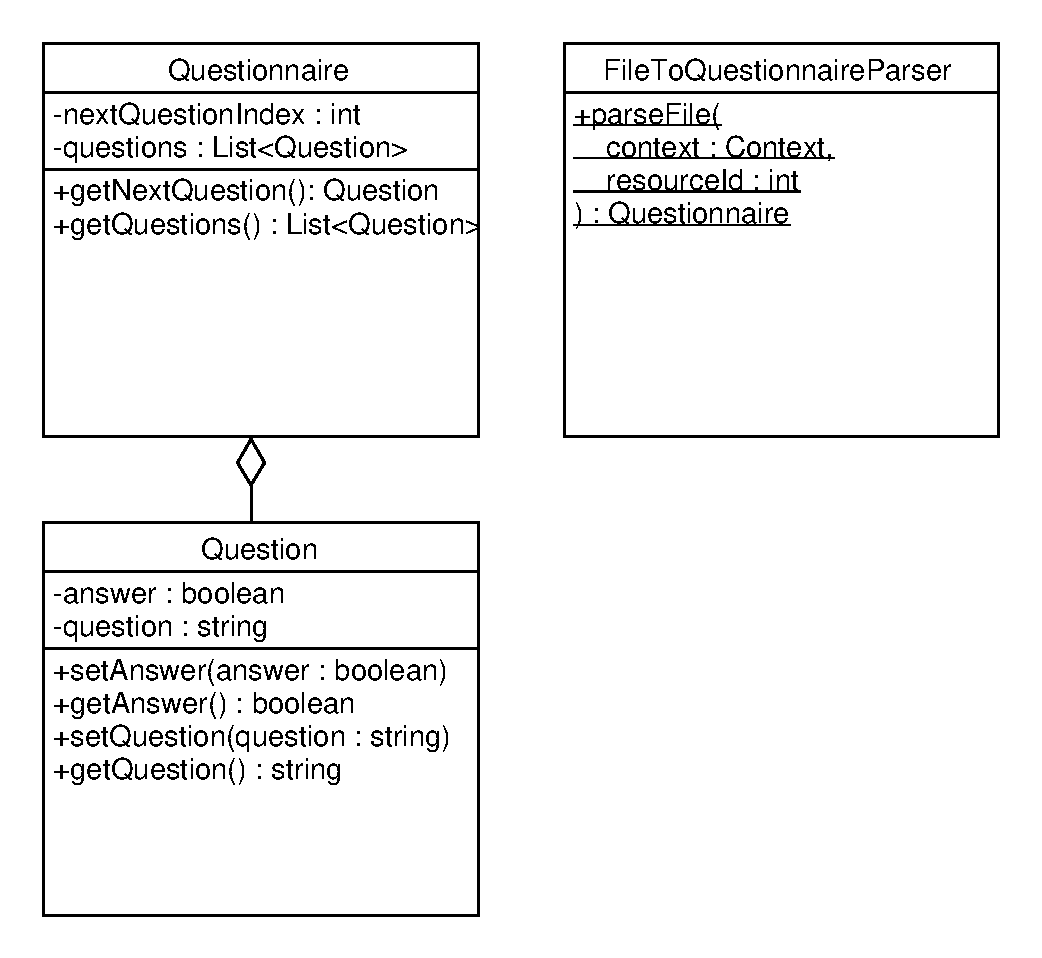
\includegraphics[width=0.6\textwidth]{graphic/data_modeling/questionnaire.pdf}
	\caption{The model of the questionnaires in the system.}
	\label{fig:questionnaire_model}
\end{figure}
\FloatBarrier

\subsection{Sensor Specification Model}
\label{sub:sensor_specification_model}

We need a nested concept or model in the \textit{campaign specification} to able to describe different parameters for the data collection from different sensors. This sensor specification model should include which sensor to sample from, the timings of when to sample data from the given sensor. 


\subsection{Campaign Class Diagram}
\label{sub:campagin_class_diagram}

Questionnaires are not the only source of data and different configurations of the different available sensors should also be customizable for customers. They should be able to specify which data sources they want to include, when they want the data gathered, and how much data they want at a time. 

\todo[inline]{ref til figur}
\begin{figure}[!htbp]
    \centering
    \includegraphics[width=\textwidth]{graphic/data_modeling/model_class_diagram.pdf}
    \caption{Class Diagram of the campaign model.}
    \label{fig:model_class_diagram}
\end{figure}
\FloatBarrier

\todo[inline]{Slut af med at vi er kommet frem til at vi skal bruge en model for det data der er blevet indsamlet og lav forward ref til snapshot sektion}

% Snapshot
%!TEX root = ../../super_main.tex

\section{Snapshot}
\label{sec:snapshot}

% Motivation 
We will also need a model for the gathered data to complement the specifications of how the individual snapshots should be composed. This model should be able handle different types of data from different sensors. Some measurements will be simple floating point numbers, to approximate real numbers, and others will consist of more complex types aggregating different values possibly of different types.  

\section{FloatTripple}
We should minimize the required storage footprint of the collected data from the data collecting application in order to minimize power consumption and thereby affecting other use of applied mobile devices as little as possible as described in \secref{sec:start_configuration}.

\todo{Beskriv FloatTripple}

% === CLIENT SERVER === %
%!TEX root = ../../super_main.tex

\chapter{Client Server Architecture}

A core features of the platform is that multiple clients should feed the server with data gathered from various context alongside labels that is derived form questionnaires. The way we handle this communication on both the client and the server is described in this chapter.

%!TEX root = ../../super_main.tex
\section{Security}


Since the system should be able to handle personal data, there are certain security constraints that we must comply with as described in \secref{sec:personal_data}. For one the legislation states that the personal data must be encrypted at all times, constraining that all ways these data are communicated must also be encrypted. For this reason we utilize an encrypted network protocol (HTTPS) using SSL encryption.

\subsection{Secure Socket Layer}
\label{sub:secure_socket_layer}
Secure Socket Layer (SSL) is a broadly used security technology for creating a secure connection between a client and a server. SSL establishes this secure connection by utilizing both symmetric and asymmetric encryption. Symmetric encryption algorithms use the same encryption key for both the encryption and decryption of the communication, whereas asymmetric encryption encrypts the communication using one key (a public key) and decrypts it using another (private key). 
\\\\
To establish the connection between the client and the server, the client initially sends the server information of how it wishes to communicate, such as what version of SSL/TLS, what cipher suites it supports and how the messages between them should be validated. The server will then chose what version and what algorithms are used in the communication and send it back to client along with its certificate and its public key. The client will then validate the certificate through a certificate authority. If it is valid the client will use the public key to encrypt a \mono{PreMasterSecret} that will be used by both the client and the server to create the key for the symmetric encryption algorithm that will be used for further information. The key will be based on both the \mono{PreMasterSecret} as well as some random numbers that have accompanied every request up to this point. The server will then decrypt the \mono{PreMasterSecret} using its private key. The server and the client can then both generate the key used for the symmetric encryption algorithm based on the random numbers and the \mono{PreMasterSecret} and use this for any further communication. 
\\\\
% self signed certificate 
% 	openssl
% ulemper ved det
% 	man in the middle vulnerability
% 	vi har været nd til at lave vores egen android stuff
% android fixes
% 	domainverifier
% 	trustmanager




\todo[inline]{Har svært ved at finde en god kilde til det her} 

%!TEX root = ../../super_main.tex
\section{Consumption of Battery and Disk}

\todo[inline]{Write about how we have prioritized the way we send data (battery vs disk)}


%!TEX root = ../../super_main.tex

\section{Restful}
Because the server is a single instance and should be able to handle a growing number of clients we must implement a communication protocol that allows to be scaled accordingly. A way to ease scalability and load balancing is to implement a restful web API, meaning that we have a uniform interface from the perspective of all devices regardless of how we choose to expand the capacity of the back end. Sophisticated tools to handle load balancing for web APIs such as Varnish \footnote{https://www.varnish-cache.org/} and HAProxy \footnote{http://www.haproxy.org/} already exist. Which effectively means that we can reduce the problem of scalability to implementing a proper Restful interface. 

\todo[inline]{Backend scalability (Restful API)}


\todo[inline]{Data sending format}

\part{Final Thoughts} 
\label{prt:final_ _thoughts_}


% === REFLECTION === %
%!TEX root = ../../super_main.tex

\chapter{Reflection}
\label{cha:reflection}

\todo[inline]{Write an introduction to the reflection chapter}

%!TEX root = ../../super_main.tex

% ==== METHOD REFLECTION ====
\section{Development Method}
Our experience shows that a user story and an acceptance test coexist in a mutual relationship. A user story draft is usually formulated first and a draft for an acceptance is then designed. The user story and acceptance test drafts are then revised back and forth until everyone claims to have understood both and have agreed on their semantics. This help us get a mutual understanding of the task and also solve potential ambiguities. 
\\\\
Another aspect that helped us clarify the intention and solve ambiguities was by estimating the user stories. 
We discovered that planning poker, which we have used to estimate tasks in iteration planning, is more valuable to us than simply being a technique for tasks estimation. Many ambiguities in task cards were discovered automatically by estimating and having short discussions about a given task. We learned that time estimation discussions quickly transformed into discussions about the semantics of the tasks when there were significant disagreements. We embraced these discussions and found that they were great means to resolve ambiguities. Time estimation discussions, when performing planning poker, are in general time boxed, but we allowed longer discussions when we felt that task cards should be updated in order to resolve ambiguities or if we felt that tasks should otherwise be split or clarified.
\\\\
Even though the discussion during estimation made the tasks more clear, it made estimation a long task. Nearing the end of the project period (approximately the last two-three iterations) the time schedule was becoming increasingly tighter, and we therefore changed from estimating all created tasks to only estimating tasks until we had enough work hours to fulfill the iteration work schedule. By making this change, we wanted the developers to feel that they were not wasting time, and we therefore embraced this shift in development methodology. Even though this change was made we still were not at a pace that would yield a product that we could be satisfied with. Therefore, the last iteration planning was made quite differently. Everyone contributed in the creation of the tasks and user stories, but when they were to be estimated, only two person was involved, whilst the other members of the group worked on the report and product. Even though it might seem controversial to estimate the task in such a way, the estimated time was close to the actual spent time. The benefit was not only that other developers could focus on other tasks during the estimation, but the time spent on the estimation was low compared to the usual planning meetings. Even though we lost the group wide discussion there were no problems with ambiguities or tasks otherwise being unclear. 
\\\\
Another aspect that worked well for us during the planning meetings was the roles that we used. 
\todo[inline]{Skriv om roller var godt}
The short iterations we used during the development have assisted with the steering of the project as was expected. It allowed us to have higher accuracy between iterations, which effectively meant that it was easier for us to focus on individual areas and know which areas needed attention, meaning that it also increased the knowledge sharing in the group. The  ceremonies that were supposed to increase the knowledge sharing in the group, namely stand up meetings and pair programming, also worked as expected. We have in earlier semesters experienced that the daily stand up meetings would over time stop being daily and later even skipped for very long periods of time. However, during this semester this has not been the case, which we believe can be contributed to the fact that we did not use a task board but rather a physical one, which was used as a center point for the meetings. 
\\\\
As mentioned in \charef{cha:development_method} we have in our project work utilized the Essence methodology. This methodology has in general helped us consider the direction of our work, and inspired discussion and reflection of how we best would solve the problem at hand. An issue that we encountered in using the essence methodology was that it would take a lot of time away from actual development and documentation of our work. This might be due to the fact that we were introduced to it this semester, meaning that we had no prior experience or knowledge about it. The fact that the course was introduced in this semester additionally meant that as the semester progressed we would be introduced to more and more concepts that might have been beneficial to have utilized in the beginning of our project. Some of these concepts included different artifacts that could have been a valuable addition to our work and report, however, at the time they were introduced it was to late to use them as intended.

\todo[color=green,inline]{Til Rikke: Er det okay at introducere en ny ting i reflektionen som vi gør her? Eller skal vi undlade det? Vi føler ikke rigtig at der er et andet godt sted i rapporten hvor vores configurations tabel kan introduceres? Hvis vi nu introducerer den her skal alle aspekter omkring den vel også introduceres i vores essence afsnit?}

One of such items were the configuration table shown in REF\todo{Smid configuration table bag i rapport og referer til den her}. We only finished this configuration table late in the project. The intended use of the table is to create one or rather evaluate and change an existing one for each iteration, however, we only finished this table nearing one of the last iterations that we had. Otherwise the table was meant to keep an overview of the different aspects of the project and should be a tool for continuously evaluating whether a project in all aspects were moving in the most optimal direction. This artifact was one of the items that we felt took a long time to create, but it still provided us with valuable insights in our project, and the time used might be reduced if we were to create one again.




%!TEX root = ../../super_main.tex

\section{The Android Platform, Compatibility and Test Driven Development}
\label{sec:the_android_platform_compatibility_and_test_driven_development}

% Uniform environment for easier knowledge sharing
%  - Android Studio
%   - code/checkstyle
%  - Phpstorm
%  - Laravel
%  - Bootstrap
%  - Jenkins
%  - Postgres

% Skriv om ovenstående her.
 

% Test
%  - Unit test
%   - Sensor data hard to mock
%  - Instrumental test 
%   - While developing -> own phones
%   - CI also requires phone
%   - Android fragmentation
%   - New OS
%    - Rooting
%    - Problems 
%    - Galaxy nexus 4.3 -> 5.0
%   - Migrating robolectric tests to instrumental




\todo[inline]{Vores temporality struktur er ikke super optimal. Fx ikke mål GPS og WiFi med samme freq som accelerometer og gyroscope. Dårlig design her: \secref{sec:structural_sensor_data}}.

% === CONCLUSION === %
%!TEX root = ../../super_main.tex

\chapter{Conclusion}
\label{cha:conclusion}


% === UNSORTED === %
%!TEX root = ../../super_main.tex

\chapter{Unsorted} 
\label{cha:unsorted}

HVOR ER DEVELOPMENT ENVIRONMENT KOMMET HEN!
% ====================== %

% \listoftodos
% \todototoc

% === Bibliografi === %
\bookmarksetup{startatroot}
\printbibliography
\label{bibliografi}
\addcontentsline{toc}{chapter}{\numberline{}Bibliography}

% === Appendix === %
% \appendix
\part{Appendicies} 
\label{prt:appendicies_}

\begin{appendices}
%!TEX root = ../../super_main.tex

%!TEX root = ../../super_main.tex
\chapter{CD}
\label{app:cd}

\dirtree{%
.1 /.
    .2 Code .
        .3 \ldots.
    .2 Report.pdf.
}
\end{appendices}

\end{document} 